%% --------------------------------------------------------------------
%% Template UTEC Tesis
%% --------------------------------------------------------------------
% Este es el archivo que se debe compilar.
% 
% Este template ha sido modificado y actualizado por Eduardo Castro y Roosevelt Ubaldo en base a lo trabajado por Víctor Murray, Oscar Ramos y Juan Carlos Barbaran.
%
% Última actualización: Mayo, 2022

\documentclass[a4paper,12pt,oneside]{tesisutec}

\selectlanguage{spanish}

%% Paquetes
\usepackage[utf8]{inputenc}
\usepackage[square, numbers, comma, sort&compress]{natbib}
% Libreria de idioma
\usepackage[spanish]{babel}
% Libreria para posicionamiento
\usepackage{float}
% Librerias para insertar codigos
\usepackage[spanish,onelanguage,ruled,vlined]{algorithm2e}
\usepackage{verbatim} 
% Librería para hipervínculos
\usepackage{hyperref}
 % Librería necesaria para arreglar el orden de referencias en overleaf.com
\usepackage{notoccite}
\usepackage{array}
\usepackage{longtable}
\usepackage{pgfgantt}
\usepackage{xcolor}
\usepackage{graphicx}
\usepackage{tikz}
\usetikzlibrary{positioning}
\usepackage{tabularx}
\usepackage{float}
\usepackage{array}
\usepackage{float}
\usepackage{array}
\usepackage{makecell}
\usepackage{longtable}
\usepackage{float}
\usepackage{ragged2e}
\renewcommand{\arraystretch}{1.4}





% Incluir acá los paquetes adicionales que deseas. 
% Ubicación de los imágenes.
\graphicspath{images/}

\makeatletter
% Reinsert missing \algbackskip
\def\algbackskip{\hskip-\ALG@thistlm}
\makeatother


\hypersetup{urlcolor=blue, colorlinks=true}
\begin{document}

\frontmatter

\department{...}
\degree{... }
\major{...}

\title{DISEÑO Y CONSTRUCCIÓN DE UN BANCO DE PRUEBAS OSCILANTE PARA VALIDACIÓN EXPERIMENTAL DE SISTEMAS MECATRÓNICOS CON SISTEMA DE ADQUISICIÓN BASADO EN ACELERÓMETROS}

\author{
    Quispe Javier, Jazmin Coral Elena~\orcid{0009-0008-8532-2215} \\
    Vera Bonilla, Ángela Milagros~\orcid{0000-0000-0000-0000}
}
% Es obligatorio agregar ORCID del alumno

\supervisor{Jara Alegria, Elvis \orcid{0000-0002-5620-7583}} % Es obligatorio agregar ORCID del asesor

\date{2025}

\maketitle

\setstretch{1.5}


% \input{encabezados/dedicatoria}
% \input{encabezados/agradecimientos}

\tableofcontents

\newpage

\listoftables

\newpage

\listoffigures

\addtocontents{toc}{\vspace{1.5em}}

%% ============================================================================
\mainmatter
\pagestyle{fancy}
%\customchapter{RESUMEN}

Este informe presenta el diseño e implementación de un banco de pruebas oscilante de 1GDL, motivado por la importancia de las pruebas de oscilación mecánica para optimizar el diseño y garantizar la integridad operativa de los sistemas, especialmente en la ingeniería mecatrónica.  El documento destaca la dificultad de predecir la respuesta de componentes y sistemas a cargas oscilatorias sin pruebas experimentales, lo que puede resultar en diseños deficientes y fallos prematuros.  

El banco de pruebas propuesto busca validar diseños y diagnosticar fallos en prototipos o componentes, sometiéndolos a condiciones oscilatorias controladas y representativas.  Se justifica su desarrollo por la necesidad de comprender y mitigar los efectos de las oscilaciones en sistemas mecatrónicos, mejorar su fiabilidad y seguridad, y abrir la puerta a futuras investigaciones en el control de oscilaciones. \\


\noindent \textbf{Palabras clave:}\\
\noindent Banco de pruebas oscilante; Sistemas mecatrónicos; Validación experimental; Oscilaciones mecánicas; Acelerómetros; Respuesta dinámica; Excitación mecánica controlada
%\customchapter{ABSTRACT} 

\begin{center}
\large \vspace{-1.5cm} \textbf{CONSTRUCTION OF THE DESIGN OF A 1DOF OSCILLATING TEST BENCH}
\end{center}

This report presents the design and implementation of a 1DOF oscillating test rig, motivated by the importance of mechanical oscillation testing to optimize design and ensure the operational integrity of systems, especially in mechatronic engineering. The paper highlights the difficulty of predicting the response of components and systems to oscillatory loads without experimental testing, which can result in poor designs and premature failures.

The proposed test rig seeks to validate designs and diagnose faults in prototypes or components by subjecting them to controlled and representative oscillatory conditions. Its development is justified by the need to understand and mitigate the effects of oscillations on mechatronic systems, improve their reliability and safety, and pave the way for future research in oscillation control.

\noindent \textbf{Keywords:}\\
\noindent Test bench; Oscillation; Mechatronic design; Validation



\customchapter{INTRODUCCIÓN} 

\introsection{Presentación del tema de investigación}

Las oscilaciones mecánicas son un fenómeno fundamental en el estudio de la dinámica de sistemas físicos, ya que afectan directamente la estabilidad, seguridad y rendimiento de estructuras y mecanismos en movimiento. Por ello es importante comprender su comportamiento para prevenir fallas estructurales, evitar resonancias indeseadas y asegurar el desempeño confiable de sistemas sometidos a estas excitaciones.

En la ingeniería mecatrónica, este análisis es aplicable en diversas áreas, como robótica, manufactura automatizada, vehículos inteligentes o maquinaria industrial, donde la interacción entre componentes mecánicos, electrónicos y de control requiere que se garantice estabilidad estructural y un desempeño dinámico confiable, razón por la que es importante integrar métodos experimentales que complementen los estudios teóricos y computacionales, para validar criterios de diseño bajo condiciones reales de operación \cite{Mikhailov2024}.


\introsection{Descripción de la situación problemática}

En muchas universidades, los proyectos desarrollados por estudiantes se evalúan únicamente mediante simulaciones computacionales, debido a la falta de infraestructura adecuada para realizar ensayos dinámicos. Como consecuencia, los diseños no son expuestos a condiciones reales de funcionamiento, lo que impide identificar fallas estructurales, inestabilidades dinámicas o deficiencias en el control. Esta situación ha sido señalada como una de las causas de desconexión entre la formación teórica y la práctica experimental en ingeniería \cite{DeLaTorre2021,Lima2017}.

A nivel regional, los países de América Latina representan solo el 2.5\,\% de la inversión mundial en investigación y desarrollo (I+D), y el 46\,\% de los investigadores iberoamericanos desarrollan sus actividades en instituciones universitarias \cite{UNESCO2024}. Esto refleja una concentración de la investigación en espacios que, en su mayoría, no cuentan con laboratorios experimentales equipados para realizar pruebas dinámicas sobre sistemas mecatrónicos en condiciones reales.

Algunas propuestas han intentado abordar este problema. Por ejemplo, en un trabajo se desarrolló un banco de pruebas para bielas basado en un mecanismo tipo inverted slider-crank, capaz de generar oscilaciones angulares con un solo grado de libertad \cite{Sevim2022}. Aunque el estudio valida experimentalmente la respuesta dinámica con herramientas accesibles como MATLAB, no integra sensores inerciales ni técnicas de análisis espectral, además de presentar una amplitud fija de oscilación, lo que limita su alcance en entornos educativos donde se busca visualizar y procesar el comportamiento físico en tiempo real. 

Asimismo, en otro proyecto se aplicó la transformada rápida de Fourier (FFT) para identificar frecuencias naturales en mecanismos oscilantes \cite{Kumari2021}, demostrando que el análisis espectral es muy útil. Sin embargo, el procesamiento frecuencial se realiza de forma aislada, sin estar integrado a plataformas que permitan observar en tiempo real. 

Adicionalmente, la mayoría de los bancos de pruebas oscilantes reportados en la literatura no incorporan mecanismos que permitan ajustar mecánicamente la amplitud de oscilación en tiempo real. Sin embargo,un estudio presentó un mecanismo tipo slider–crank ajustable mediante la guía del deslizador, lo que permite modificar la trayectoria angular, y por tanto la amplitud, sin alterar la frecuencia de operación \cite{cheng2001adjustable}. Este enfoque es relevante en entornos educativos, pero no considera la integración de sensores inerciales como acelerómetros ni el análisis frecuencial, lo cual limita su aplicación en un contexto real donde se quiere caracterizar la dinámica del sistema.

En conjunto, esto permitiría analizar dinámicamente el sistema desde fases tempranas, facilitando la detección de problemas funcionales que, según estudios, explican más del 40\% de las fallas en proyectos mecatrónicos durante esta fase \cite{Haas2024}. 


\introsection{Formulación del problema}

A partir de esta problemática, se definió la siguiente pregunta:

\begin{quote}
\textbf{¿Cómo pueden obtenerse datos confiables sobre el comportamiento dinámico de prototipos mecatrónicos en entornos académicos, mediante un sistema que permita aplicar y medir oscilaciones mecánicas controladas?}
\end{quote}

\introsection{Objetivos de investigación}

\textbf{Objetivo General:}

Diseñar y construir un banco de pruebas oscilante de dos grados de libertad (GDL) que permita validar la respuesta dinámica de componentes mecatrónicos en un entorno académico controlado.

\textbf{Objetivos Específicos}:
\begin{itemize}
\item [1.] Diseñar el sistema mecánico y de actuación del banco de pruebas, considerando la posibilidad de ajustar parámetros como frecuencia y amplitud de oscilación.

\item [2.] Desarrollar e implementar un sistema de adquisición y medición de vibraciones basado en acelerómetros, adecuado para entornos académicos.

\item [3.] Desarrollar una interfaz de usuario que permita configurar los parámetros de excitación y visualizar los datos adquiridos en tiempo real.

\item [4.] Caracterizar experimentalmente las oscilaciones generadas bajo diferentes condiciones de carga, frecuencia y amplitud, utilizando técnicas de análisis de Fourier para evaluar la respuesta en frecuencia.
\end{itemize}



\introsection{Justificación}

El desarrollo de un banco de pruebas oscilante de 2 grados de libertad (2 DoF) surge como una respuesta a la limitada capacidad que tienen muchas instituciones académicas para validar dinámicamente prototipos mecatrónicos. En la práctica, esto genera una brecha entre la simulación y la prueba física, dificultando la detección oportuna de fallos estructurales o deficiencias en el diseño.

La solución propuesta busca cubrir la necesidad de una plataforma mecánica que permita generar oscilaciones de forma controlada, con una amplitud de oscilación variable y la observación directa de la respuesta dinámica ante diferentes condiciones de carga, frecuencia y amplitud, sin requerir sistemas complejos.

Además, permitirá realizar prácticas experimentales con sensores inerciales y análisis espectral en tiempo real, fortaleciendo la adquisición de datos, procesamiento y diagnóstico dinámico. Esto no solo complementa el aprendizaje teórico, sino que también ofrece a los estudiantes una herramienta concreta para validar y mejorar sus propios diseños.


\introsection{Alcance y limitaciones / restricciones}

El sistema propuesto permitirá aplicar oscilaciones mecánicas controladas y registrar la respuesta dinámica mediante sensores inerciales MEMS, como se investigó en los antecedentes. Se empleará un mecanismo tipo \emph{inverted slider-crank} para generar el movimiento, el cual tendrá un ajuste regulable de amplitud de oscilación, junto con un sistema de adquisición basado en acelerómetros montados en puntos clave. Se desarrollará una interfaz de usuario en una pantalla aparte empleando ESP32 el cual permitirá ajustar el tiempo de duración de la prueba, además de incorporar controles básicos como amplitud y frecuencia. 

El análisis se realizará en el dominio de la frecuencia mediante la transformada rápida de Fourier. Además de incluirse control activo para regular su comportamiento. En una etapa posterior, se contempla incorporar sensores adicionales para medir corriente, potencia y fuerza, con el fin de complementar la caracterización dinámica, además de dejarse abierta la posibilidad de emplear IMUS en futuras etapas.

El banco de pruebas no está orientado a aplicaciones industriales. Su diseño está pensado para un entorno académico, con condiciones de prueba seguras. No se considera su uso en exteriores, con cargas elevadas o bajo perturbaciones ambientales severas.

Las condiciones como temperatura o humedad no serán monitoreadas ni controladas, asumiendo que su efecto es mínimo para los fines educativos propuestos. Finalmente, la plataforma está destinada a actividades de formación, por lo que su precisión y capacidades estarán alineadas con los requerimientos de laboratorio universitario, no de sistemas industriales.




\chapter{REVISIÓN CRÍTICA DE LA LITERATURA}

A pesar de la limitada literatura directamente relacionada con la problemática abordada, se identificaron trabajos que respaldan aspectos clave de la solución propuesta. Estos estudios aportan en el diseño de sistemas oscilantes, el uso de bancos de prueba, la selección de actuadores, la medición dinámica con sensores y el análisis espectral de oscilaciones, proporcionando así una base sólida para el desarrollo de la tesis.

El estudio de las oscilaciones mecánicas es importante para entender y validar la respuesta dinámica de las estructuras. En ese sentido, diversos estudios abordaron la implementación de mecanismos oscilantes en entornos experimentales. Por ejemplo, un trabajo describe un sistema de fatiga torsional basado en un motor y un volante acoplado a un resorte, generando oscilaciones angulares controladas \cite{pena2012}. De forma similar, se propone un banco torsional con excitación mixta DC+AC \cite{patil2013}. Ambos estudios refuerzan la validez de usar mecanismos sencillos para inducir oscilaciones, los cuales destacan por su ser simples y fáciles de replicar, aunque presentan limitaciones en cuanto a flexibilidad de control y escalabilidad para distintas geometrías de prueba.

Asimismo, la existencia de bancos de prueba validados en laboratorio permite tomar como referencia sus diseños estructurales y metodologías de ensayo. Un estudio describe un banco de pruebas para bielas impulsado por un mecanismo de manivela, el cual comparte similitudes cinemáticas con la configuración tipo \emph{inverted slider-crank} \cite{Sevim2022}. Este mecanismo, como se observa en la figura \ref{fig:mec_invvvv}, emplea un motor asíncrono con reducción y usa encoders para registrar velocidad; además plantea un análisis dinámico detallado a través de la ecuación de Lagrange, considerando efectos de masa e inercia, y se valida experimentalmente mediante un codificador óptico. Se evidencia una fluctuación del 20\% en la velocidad del cigüeñal debido a la variación del momento de inercia durante el ciclo, lo que pone en relevancia el comportamiento dinámico no lineal del sistema. Este aporte resulta especialmente valioso para la propuesta, ya que sustenta la pertinencia de emplear mecanismo del tipo \emph{inverted slider-crank} con trayectorias oscilantes generadas mecánicamente. Además, demuestra la viabilidad de su análisis mediante herramientas accesibles como MATLAB. Su principal debilidad es que no aborda el procesamiento de señales ni el uso de sensores adicionales, pero su valor técnico como antecedente de estructura y funcionamiento es clave para la solución propuesta, además de no permitir regulación de sus parámetros de operación como amplitud.

\begin{figure}[H]
\begin{center}
\includegraphics[width=0.7\textwidth]{images/inverted.png}
\caption{Mecanismo experimental de tipo inverted slider-crank}
\label{fig:mec_invvvv}
\end{center}
\end{figure} 

En la literatura también se han explorado sistemas de excitación mediante motores DC acoplados a levas o excéntricos \cite{filippatos2019}, resortes torsionales \cite{patil2013}, y actuadores piezoeléctricos \cite{wang2020}. La tabla \ref{tab:oscilaciones} resume estas configuraciones, donde se destaca que sistemas mecánicos como leva-eje son efectivos en generar oscilaciones periódicas. La fortaleza de estas propuestas es su variedad de principios de actuación, lo que permite compararlas según el requerimiento de frecuencia y amplitud. No obstante, muchas de ellas requieren controladores especializados o estructuras complejas no compatibles con la propuesta y objetivos del proyecto.

\begin{table}[H]
\centering
\begin{tabular}{|p{2.2cm}|p{3cm}|p{3cm}|p{3cm}|p{3cm}|}
\hline
\textbf{Autor / Referencia} & \textbf{Actuador y configuración mecánica} & \textbf{Tipo de oscilación} & \textbf{Forma de control} & \textbf{Observaciones} \\
\hline
Filippatos et al. (2019) \cite{filippatos2019} & Motor DC + leva acoplada a masa o brazo & Angular o lineal periódica & PWM o perfil de leva prediseñado & Bajo costo, frecuencia fija o semivariable \\
\hline
Patil y Teodoriu (2013) \cite{patil2013} & Motor DC/AC con resorte torsional acoplado a eje & Angular resonante & Señal senoidal + adquisición de torque & Buen desempeño en frecuencias naturales \\
\hline
Wang et al. (2020) \cite{wang2020} & Actuador piezoeléctrico unimorfo/bimorfo sobre viga delgada & Micrométrica transversal & Señal senoidal de alta tensión (HV driver) & Precisión elevada, desplazamientos pequeños \\
\hline
Sevim y Uzmay (2022) \cite{Sevim2022} & Motor asíncrono + reductor + mecanismo tipo \emph{inverted slider-crank} & Angular oscilante (±45°) & Velocidad fija + medición mediante encoder & 1 DOF, validación experimental, oscilación mecánica pura \\
\hline
\end{tabular}
\caption{Resumen de configuraciones para la generación de oscilaciones mecánicas}
\label{tab:oscilaciones}
\end{table}

También se han presentado mecanismos que permiten ajustar la amplitud de oscilación en bancos de prueba, aunque con distintas limitaciones. Por ejemplo, en un trabajo se propuso una configuración de tipo \emph{slider–crank} con guía móvil, la cual permite variar la amplitud de forma manual al modificar la posición del deslizador dentro del mecanismo \cite{cheng2001adjustable}. Esta estrategia posibilita generar diferentes trayectorias sin alterar la velocidad de entrada, aunque no contempla la incorporación de sensores inerciales ni análisis dinámico. 

Por otro lado, otro estudio modeló un excitador mecánico también basado en un slider–crank, en el que la amplitud se ajusta modificando los parámetros geométricos del sistema, tales como las longitudes de los eslabones o el ángulo de entrada \cite{korendiy2024}. Si bien su enfoque permite analizar distintas condiciones cinemáticas mediante simulación, el estudio no desarrolla un prototipo físico ni considera la adquisición de datos en tiempo real. Adicionalmente, como se observa en la figura \ref{fig:ajust}, se diseñó un banco con un actuador lineal acoplado al mecanismo, que permite modificar electrónicamente la posición del deslizador y, con ello, ajustar la amplitud de oscilación durante la operación \cite{lanets2021}. Aunque este diseño incorpora control activo, está orientado a entornos industriales y no incluye sensado inercial ni procesamiento espectral integrado. En conjunto, estos trabajos muestran diferentes maneras de regular la amplitud mecánica, pero también evidencian vacíos respecto a la integración de elementos de medición y análisis dinámico que permitan caracterizar el comportamiento oscilatorio en tiempo real, especialmente en contextos académicos.

\begin{figure}[H]
\begin{center}
\includegraphics[width=0.7\textwidth]{images/amplitudajustable.png}
\caption{Diagrama de la estructura del mecanismo usado para generar oscilaciones en la máquina vibratoria}
\label{fig:ajust}
\end{center}
\end{figure} 

Debido a esta razón, además de los actuadores, se requieren sensores para caracterizar dinámicamente las oscilaciones, varios autores han demostrado que el uso de acelerómetros es una alternativa confiable para monitorear vibraciones y oscilaciones en sistemas dinámicos. Por ejemplo, un trabajo reciente caracterizó acelerómetros MEMS a bajas frecuencias en una plataforma oscilante, obteniendo alta resolución en la medición de desplazamientos lineales inducidos por un excitador electromagnético tipo altavoz \cite{srokosz2024}. En dicho estudio, se utilizó una bobina móvil montada sobre una base rígida, excitada mediante señales generadas por un DAC de 16 bits, logrando oscilaciones de hasta ±10 mm entre 0.001 y 2000 Hz. Además, se integraron sensores inerciales que retroalimentaban el sistema en tiempo real, permitiendo el ajuste dinámico mediante transformada rápida de Fourier (FFT) para mantener la estabilidad de la oscilación. Como conclusión del trabajo, se validó que varios sensores de bajo costo como MPU6050, MPU6500 y ADXL345 son adecuados para tareas de monitoreo dinámico en entornos estructurales. A pesar de no ser los más avanzados, estos modelos cumplen con criterios de estabilidad operativa, sensibilidad y eficiencia energética, siempre que se apliquen metodologías de prueba y calibración apropiadas.

De forma complementaria, otros estudios han explorado el uso de sensores MEMS en entornos experimentales para análisis vibratorio. Un trabajo validó una plataforma que emplea acelerómetros MEMS de bajo costo para el monitoreo estructural \cite{Cocconcelli2015}, demostrando su aplicabilidad en tareas de diagnóstico dinámico. Destacando su fácil implementación y relación costo-beneficio, aunque también identifican limitaciones asociadas a la resolución, ruido electrónico y necesidad de calibración según el entorno de uso.


Por otro lado, el análisis espectral mediante la transformada rápida de Fourier (FFT) se ha consolidado como una herramienta robusta y replicable para el diagnóstico de comportamientos dinámicos. Sin embargo, en escenarios donde se requiere mayor precisión, versiones mejoradas como la e‑FFT (enhanced FFT) han demostrado un rendimiento superior. Estas variantes permiten incrementar la resolución espectral y reducir significativamente el error en la estimación de la frecuencia y amplitud de componentes armónicas, como se evidenció en el monitoreo de rodamientos instrumentados con acelerómetros \cite{Lin2016, Lin2019}. Gracias a técnicas de interpolación y refinamiento espectral, la e‑FFT logró detectar variaciones menores a ±0.5 Hz y mejorar la estimación de amplitud en entornos con ruido, como se observa en la figura \ref{fig:fft}.

\begin{figure}[H]
\begin{center}
\includegraphics[width=0.7\textwidth]{images/fftvse-fft.jpg}
\caption{Comparativa espectro frecuencia con FFT y e-FFT}
\label{fig:fft}
\end{center}
\end{figure} 

Asimismo, la transformada de Fourier ha sido aplicada para reconstruir desplazamientos a partir de señales cuasi‑periódicas, logrando mitigar la deriva acumulada con errores inferiores a ±9 mm \cite{Sabatini2015}. Esta estrategia resulta especialmente útil cuando se requiere caracterizar trayectorias oscilantes con precisión a partir de datos de aceleración. En un contexto educativo, también se ha implementado un sistema experimental de bajo costo que identificó la frecuencia natural (17 Hz) de un mecanismo oscilante utilizando FFT en LabVIEW, demostrando su viabilidad tanto para validación dinámica como para formación técnica \cite{Kumari2021}.

En conjunto, estos enfoques respaldan que la integración de sensores inerciales como acelerómetros MEMS con el análisis espectral mediante FFT constituye una metodología sólida, económica y replicable para el estudio dinámico de mecanismos oscilantes. Esta combinación permite identificar de manera confiable las frecuencias características del sistema y monitorear su comportamiento operativo. En el contexto de la solución propuesta, como se mencionó párrafos atrás, se destaca que sea basado en el tipo inverted slider-crank con amplitud de oscilación ajustable, el cual permite validar la respuesta del mecanismo, siendo además escalable hacia técnicas de mayor resolución como la e‑FFT si se requiere un análisis más detallado en futuras etapas.

\chapter{MARCO TEÓRICO}

A partir de la revisión crítica de literatura, se identificaron tres componentes clave: oscilaciones mecánicas, banco de pruebas oscilante y análisis frecuencial (FFT). Estos fundamentos respaldan el diseño del banco de pruebas desarrollado y sirven como base para interpretar sus resultados.


\section{Oscilaciones mecánicas}

Las oscilaciones mecánicas (movimientos periódicos alrededor de una posición de equilibrio en sistemas masa–resorte–amortiguador) son ampliamente estudiadas para el análisis de respuesta dinámica y validación de sistemas mecatrónicos \cite{mit_ocw_second_order, sciencedirect_second_order}. Cuando una fuerza externa desplaza el sistema, la rigidez y la inercia provocan retornos sucesivos, generando oscilaciones libres o forzadas \cite{mit_second_order_response}.

La dinámica está descrita por:

\begin{equation}
\label{eq:ecuacion_dinamica}
m\ddot{x}(t) + c\dot{x}(t) + kx(t) = F(t)
\end{equation}

Dividiendo por \(m\), se definen la frecuencia natural \(\omega_n\) y el coeficiente de amortiguamiento relativo \(\zeta\) \cite{sciencedirect_second_order}:

\begin{equation}
\label{eq:frecuencia_amortiguamiento}
\omega_n = \sqrt{\frac{k}{m}}, \quad \zeta = \frac{c}{2\sqrt{km}}
\end{equation}

Según el valor de \(\zeta\) de la ecuación \ref{eq:frecuencia_amortiguamiento}, el sistema se comporta de forma diferente:

\begin{itemize}
    \item Si \(\zeta < 1\): sistema subamortiguado, con oscilaciones amortiguadas:
    \[
    x(t) = A e^{-\zeta \omega_n t} \cos(\omega_d t + \phi), \quad \omega_d = \omega_n \sqrt{1 - \zeta^2}
    \]
    \item Si \(\zeta = 1\): amortiguamiento crítico, sin oscilaciones.
    \item Si \(\zeta > 1\): sobreamortiguado, respuesta lenta sin oscilaciones.
\end{itemize}

El análisis en el dominio de la frecuencia, utilizando herramientas como la transformada de Fourier, permite identificar frecuencias naturales y evaluar resonancias \cite{mit_ocw_second_order}.

\subsection{Excitación mecánica controlada}

La excitación mecánica controlada se refiere a la aplicación deliberada de movimientos oscilatorios en un sistema mediante actuadores, con el fin de inducir una respuesta medible. Dependiendo del tipo de actuador, se pueden generar perfiles periódicos como ondas sinusoidales, cuadradas o personalizadas \cite{mit_mechatronics_modeling}.

Los actuadores comúnmente utilizados incluyen motores eléctricos (DC, paso a paso), motores con reductores, actuadores lineales y, en aplicaciones más precisas, dispositivos piezoeléctricos. La elección del actuador depende del tipo de oscilación deseada (angular o lineal), la frecuencia objetivo, la carga a mover y el grado de control necesario.

En el presente proyecto se emplea una configuración mecánica que transforma el movimiento rotativo de un motor en oscilación angular, lo que permite generar perfiles repetitivos de manera controlada.

\section{Banco de pruebas oscilante}

Un banco de pruebas oscilante es una plataforma diseñada para inducir oscilaciones mecánicas controladas en sistemas mecatrónicos, permitiendo estudiar parámetros dinámicos como frecuencia natural, rigidez y amortiguamiento \cite{construction_impedance_bench, multifunc_test_bench}. Se utilizan ampliamente en investigación, validación de algoritmos y docencia.

\textbf{Dificultades comunes}:

\begin{itemize}
    \item Precisión del montaje y aislamiento de vibraciones externas
    \item Ruido en los sensores
    \item Calibración de los actuadores
    \item Seguridad frente a resonancia y fatiga mecánica
\end{itemize}

Suelen emplearse en aplicaciones de laboratorio para la enseñanza de dinámica estructural, validación de sensores, o evaluación de componentes mecatrónicos. Un banco de pruebas debe permitir la medición fiable de variables como aceleración, desplazamiento y fuerza, además de ofrecer seguridad ante posibles resonancias o fallas estructurales.

\subsection{Sistema mecánico y de actuación}

El mecanismo propuesto para el banco de pruebas oscilante está constituido por cinco eslabones conectados mediante pares cinemáticos revoluta y prismática, conformando un sistema plano de dos grados de libertad.

\begin{figure}[H]
\begin{center}
\includegraphics[width=0.9\textwidth]{images/cinematica.jpg}
\caption{(a) Diagrama del mecanismo  (b) Diagrama vectorial del mecanismo}
\label{fig:cinmatica}
\end{center}
\end{figure}


El movimiento del conjunto es inducido por un motor ubicado en el punto A, el cual aplica un momento torsor sobre el primer eslabón móvil, una biela motriz articulada al bastidor mediante un par revoluta. Esta biela transmite el movimiento a un eslabón intermedio a través de una segunda articulación rotacional. El eslabón intermedio funciona como acoplador, cuya función es transferir la energía cinemática hacia el siguiente componente del sistema mediante un enlace prismático, que permite un desplazamiento lineal relativo entre ambos cuerpos a lo largo de una dirección fija.

El cuarto eslabón del sistema actúa como oscilador, ejecutando un movimiento angular alternante respecto a una dirección de referencia determinada por las condiciones geométricas del sistema. Este oscilador se encuentra vinculado al eslabón de cierre por medio de un segundo par prismático. Este último enlace cumple una función esencial: permite regular la amplitud de oscilación del eslabón oscilante. Al modificar la posición relativa entre los puntos de acoplamiento prismáticos, se altera la configuración geométrica del mecanismo, afectando directamente el ángulo máximo alcanzado por el oscilador durante su movimiento cíclico.


\subsubsection{Configuración del mecanismo}

El mecanismo analizado corresponde a un sistema de cinco barras dispuestas de forma que forman dos lazos cerrados, incluyendo un cuerpo rígido en forma de "L". Este cuerpo está formado por las barras $r_4$ y $r_5$, unidas en ángulo recto. Se consideran los siguientes elementos:

\begin{itemize}
\item $d$: distancia fija entre los pivotes A y D (base).
\item $a$: biela de entrada (manivela), que gira con $\theta_2$.
\item $b$: barra intermedia que conecta el punto B con C.
\item $e$: parte horizontal del cuerpo en L (de C hacia P).
\item $c$: parte vertical del cuerpo en L (de D hacia E), donde se instala un actuador de longitud constante.
\end{itemize}

La secuencia de puntos sigue el orden: A $\rightarrow$ B $\rightarrow$ C $\rightarrow$ E $\rightarrow$ D. El punto P se encuentra en la prolongación de la barra horizontal desde C. El cuerpo CE–ED se comporta como una pieza rígida unificada.

\subsubsection{Análisis de posición}

Este análisis tiene como objetivo determinar la orientación angular $\theta_3$ del cuerpo rígido, así como la posición de los puntos C, E y P a partir de los valores conocidos de $\theta_2$ y las longitudes geométricas.

\textbf{Cierre vectorial} \\

Se emplea una ecuación de cierre vectorial que representa el lazo del mecanismo:
\begin{equation}
\vec{r}_2 + \vec{r}_3 + \vec{r}_4 = \vec{r}_1 + \vec{r}_5
\end{equation}

Reorganizando:
\begin{equation}
\vec{r}_3 + \vec{r}_4 + \vec{r}_5 = \vec{b}, \quad \text{donde } \vec{b} = -\vec{r}_1 - \vec{r}_2
\end{equation}

Cada vector se expresa en coordenadas cartesianas, considerando que $\theta_3$ es el ángulo del cuerpo rígido CE respecto al eje horizontal:
\begin{align}
\vec{r}_3 &= r_3 \begin{bmatrix} \cos\theta_3 \ \sin\theta_3 \end{bmatrix}, &
\vec{r}_4 &= r_4 \begin{bmatrix} \sin\theta_3 \ -\cos\theta_3 \end{bmatrix}, \\
\vec{r}_5 &= r_5 \begin{bmatrix} -\cos\theta_3 \ -\sin\theta_3 \end{bmatrix}
\end{align}

Sumando estos vectores obtenemos:
\begin{equation}
\vec{b} = (r_3 - r_5) \begin{bmatrix} \cos\theta_3 \ \sin\theta_3 \end{bmatrix} + r_4 \begin{bmatrix} \sin\theta_3 \ -\cos\theta_3 \end{bmatrix}
\end{equation}

\textbf{Solución analítica} \\

Separando en componentes $x$ e $y$ del vector $\vec{b}$:
\begin{align}
b_x &= r_4 \sin\theta_3 + (r_3 - r_5) \cos\theta_3 \
b_y &= -r_4 \cos\theta_3 + (r_3 - r_5) \sin\theta_3
\end{align}

Despejando $\theta_3$ de manera analítica:
\begin{equation}
\theta_3 = \tan^{-1} \left( \frac{(r_3 - r_5)b_y + b_x}{(r_3 - r_5)b_x - b_y} \right)
\end{equation}

\subsubsection{Análisis de velocidad}

El análisis de velocidad permite determinar las velocidades angulares y lineales de los eslabones, especialmente la velocidad angular del cuerpo rígido CE y la velocidad del punto P.

\begin{equation}
\vec{v}_3 + \vec{v}_4 + \vec{v}_5 = \vec{v}_b = -\vec{v}_2
\end{equation}

Expresando cada vector de velocidad en función de las velocidades angulares:
\begin{align}
\vec{v}_2 &= r_2 \omega_2 \begin{bmatrix} -\sin\theta_2 \ \cos\theta_2 \end{bmatrix}, \\
\vec{v}_3 &= r_3 \omega_3 \begin{bmatrix} -\sin\theta_3 \ \cos\theta_3 \end{bmatrix}, \\
\vec{v}_4 &= r_4 \omega_3 \begin{bmatrix} \cos\theta_3 \ \sin\theta_3 \end{bmatrix}, \\
\vec{v}_5 &= r_5 \omega_3 \begin{bmatrix} \sin\theta_3 \ -\cos\theta_3 \end{bmatrix}
\end{align}

Resolviendo en componentes se obtiene el valor de $\omega_3$.

\subsubsection{Análisis de aceleración}

Se realiza la derivación de las velocidades para obtener las aceleraciones lineales de cada eslabón:

\begin{equation}
\vec{a}_3 + \vec{a}_4 + \vec{a}_5 = \vec{a}_b = -\vec{a}_2
\end{equation}

Donde cada aceleración tiene componentes tangenciales y centrípetas:
\begin{align}
\vec{a}_2 &= r_2 \alpha_2 \begin{bmatrix} -\sin\theta_2 \ \cos\theta_2 \end{bmatrix} - r_2 \omega_2^2 \begin{bmatrix} \cos\theta_2 \ \sin\theta_2 \end{bmatrix}, \\
\vec{a}_3 &= r_3 \alpha_3 \begin{bmatrix} -\sin\theta_3 \ \cos\theta_3 \end{bmatrix} - r_3 \omega_3^2 \begin{bmatrix} \cos\theta_3 \ \sin\theta_3 \end{bmatrix}, \\
\vec{a}_4 &= r_4 \alpha_3 \begin{bmatrix} \cos\theta_3 \ \sin\theta_3 \end{bmatrix} - r_4 \omega_3^2 \begin{bmatrix} -\sin\theta_3 \ \cos\theta_3 \end{bmatrix}, \\
\vec{a}_5 &= r_5 \alpha_3 \begin{bmatrix} \sin\theta_3 \ -\cos\theta_3 \end{bmatrix} - r_5 \omega_3^2 \begin{bmatrix} \cos\theta_3 \ \sin\theta_3 \end{bmatrix}
\end{align}

\subsubsection{Análisis cinético}

\begin{figure}[H]
\begin{center}
\includegraphics[width=0.7\textwidth]{images/CINETICA1.png}
\caption{Mecanismo de cinco barras accionado por el momento M2}
\label{fig:cinmatica2}
\end{center}
\end{figure}

Se incluye la rotación de los eslabones y el desplazamiento del punto P:

\begin{equation}
T = \frac{1}{2} I_2 \omega_2^2 + \frac{1}{2} I_3 \omega_3^2 + \frac{1}{2} m_4 v_P^2 + \frac{1}{2} I_4 \omega_3^2
\end{equation}

Donde:
\begin{itemize}
\item $I_i$: momentos de inercia de los eslabones alrededor de su centro de masa.
\item $v_P$: velocidad absoluta del punto extremo P.
\end{itemize}

\textbf{Ecuaciones de equilibrio dinámico del mecanismo de cinco barras} \\

\begin{figure}[H]
\begin{center}
\includegraphics[width=0.7\textwidth]{images/CINETICA2.png}
\caption{Diagramas de cuerpo libre para eslabones sometidos a fuerzas a lo largo del eslabón en un mecanismo de cinco barras.}
\label{fig:cinmatica3}
\end{center}
\end{figure}

\begin{figure}[H]
\begin{center}
\includegraphics[width=0.7\textwidth]{images/CINETICA3.png}
\caption{Diagramas de cuerpo libre para eslabones sometidos a fuerzas normales al eslabón en un mecanismo de cinco barras}
\label{fig:cinmatica2}
\end{center}
\end{figure}

En esta sección se consideran las fuerzas de inercia significativas que actúan sobre los eslabones, de acuerdo con el modelo desarrollado en la Sección 3.5.4 del texto de referencia. Se asume que no hay fuerzas de fricción y que el sistema tiene un actuador lineal fijo en longitud en la barra vertical (Eslabón 5).

\textbf{Eslabón 2:}
\begin{align}
F_{12}^{\eta} + F_{32}^{\eta} + P_2^{\eta} &= 0 \\
-r_2 F_{12}^{\eta} - M_2 + M_2^i - r_{c2} P_2^{\eta} &= 0 \\
F_{12}^{\eta} &= \frac{-M_2 + M_2^i - r_{c2} P_2^{\eta}}{r_2} \\
F_{32}^{\eta} &= -P_2^{\eta} - F_{12}^{\eta}
\end{align}

\textbf{Eslabón 3:} (sin reacciones normales si no hay fricción)

\textbf{Eslabón 4 (cuerpo CE):}
\begin{align}
F_{34}^{\eta} - F_{54}^{\eta} + P_4^{\eta} - P_4 &= 0 \\
-r_{c3} F_{34}^{\eta} + M_4^i - r_{c4} P_4^{\eta} + M_{54} + r_{D4} P_4 &= 0 \\
F_{34}^{\eta} &= \frac{M_{54} + M_4^i - r_{c4} P_4^{\eta} + r_{D4} P_4}{r_4} \\
F_{54}^{\eta} &= P_4^{\eta} + F_{34}^{\eta} - P_4
\end{align}

\textbf{Eslabón 5 (barra DE):}
\begin{align}
-F_{15}^{\eta} + P_5^{\eta} &= 0 \\
M_5^i - r_{c5} P_5^{\eta} - M_{54} &= 0 \\
M_{54} &= M_5^i - r_{c5} P_5^{\eta} \\
F_{15}^{\eta} &= P_5^{\eta}
\end{align}

\textbf{Análisis de fuerzas longitudinales (dirección )} \\

\textbf{Eslabón 2:}
\begin{equation}
-F_{12}^{\xi} + F_{32}^{\xi} = 0
\end{equation}

\textbf{Eslabón 3:}
\begin{equation}
-F_{23}^{\xi} + F_{43}^{\xi} - P_3^{\xi} = 0
\end{equation}

\textbf{Eslabón 4:} No tiene fuerzas longitudinales si no hay fricción.

\textbf{Eslabón 5:}
\begin{equation}
F_{15}^{\xi} - F_{54}^{\xi} - P_5^{\xi} = 0
\end{equation}

\textbf{Cálculo de la fuerza de resistencia } \\

Las fuerzas internas son funciones de la fuerza de resistencia externa . Según el equilibrio de momentos:
\begin{align}
F_{34}^{\eta} &= \frac{M_{54} + M_4^i - r_{c4} P_4^{\eta} + r_{D4} P_4}{r_4} \\
F_{54}^{\eta} &= \frac{M_5^i + M_4^i + (r_4 - r_{c4}) P_4^{\eta} + r_{D4} P_4}{r_4}
\end{align}

\textbf{Fuerzas internas:}
\begin{align}
F_{32}^{\xi} &= -F_{34}^{\xi} \cot(\theta_3 - \theta_2) \\
F_{32}^{\eta} &= \frac{F_{34}^{\xi}}{\sin(\theta_3 - \theta_2)} \\
P_4 &= \frac{r_4}{r_{D4}} (M_5^i - M_4^i + r_{c4} P_4^{\eta} - r_{D4} P_4^{\eta} - F_{32}^{\xi} \sin(\theta_3 - \theta_2))
\end{align}

\textbf{Transformación a coordenadas globales:}
\begin{equation}
\vec{F}{12} = -F{12}^{\xi} [\cos\theta_2, \sin\theta_2]^T + F_{12}^{\eta} [-\sin\theta_2, \cos\theta_2]^T
\end{equation}

Estas expresiones completan el análisis dinámico considerando las fuerzas normales y longitudinales aplicadas a cada eslabón del mecanismo, y permiten calcular las fuerzas internas y externas en función de las condiciones dinámicas del sistema.

\subsection{Acelerómetros}

Un acelerómetro mide aceleración detectando la fuerza inercial que actúa sobre una masa suspendida cuando el sensor está sometido a movimiento \cite{rg_memscap_review, sciencedirect_accelerometer}. Este principio sigue la segunda ley de Newton: 

\begin{equation}
F = ma
\label{eq:newton}
\end{equation}

Las tecnologías principales incluyen:

\begin{itemize}
    \item \textbf{Capacitivos (MEMS)}: miden el cambio de capacitancia \(C = \varepsilon A / d\) debido al desplazamiento causado por aceleración \cite{rg_memscap_review, sciencedirect_new_capsensor}.
    \item \textbf{Piezoeléctricos}: generan una carga eléctrica \(Q = d_{33} \cdot F\) al aplicarse una fuerza sobre un cristal \cite{mdpi_piezo_review, nature_pvdf_accelerometer}.
    \item \textbf{Piezoresistivos}: la aceleración produce deformaciones que alteran la resistencia, medida mediante un puente de Wheatstone \cite{pmc_wearable_piezoresistive}.
\end{itemize}

La velocidad se calcula integrando la aceleración:

\begin{equation}
v(t) = \int a(t) \, dt
\label{eq:velocidad}
\end{equation}

En el contexto del presente proyecto, se emplean acelerómetros MEMS (Micro Electro Mechanical Systems) debido a su bajo costo, tamaño compacto y facilidad de integración en entornos académicos. Estos sensores son capaces de registrar las oscilaciones generadas por el mecanismo, permitiendo así obtener datos útiles para el análisis espectral y la validación experimental.

\begin{figure}[H]
\centering
\includegraphics[width=0.55\textwidth]{images/principio_acelerometro.png}
\caption{Esquema básico de funcionamiento de un acelerómetro tipo MEMS capacitivo \cite{sciencedirect_accelerometer}.}
\label{fig:acelerometro_mem}
\end{figure}


\textbf{Dificultades comunes} 

A pesar de sus ventajas, los acelerómetros MEMS presentan limitaciones que deben considerarse en el diseño experimental:

\begin{itemize}
\item Deriva en mediciones prolongadas (especialmente al integrar para obtener velocidad o desplazamiento).
\item Sensibilidad a la orientación y temperatura \cite{ml_temperature_comp2021}.
\item Saturación en frecuencias altas y presencia de ruido electrónico.
\end{itemize}

En este proyecto, estos efectos serán minimizados mediante una correcta selección del rango dinámico, uso de filtros digitales y configuración del sensor en el eje dominante de la oscilación.

\section{Transformada de Fourier y análisis en frecuencia}

La transformada de Fourier (TF) permite representar una señal temporal en términos de sus componentes frecuenciales, lo cual es esencial en el análisis de oscilaciones. Esta herramienta es ampliamente utilizada para identificar frecuencias naturales, modos de resonancia y comportamiento dinámico de estructuras sometidas a excitaciones periódicas \cite{Inman2013}.

La expresión general para la TF de una señal continua $x(t)$ es:

\begin{equation}
X(f) = \int_{-\infty}^{\infty} x(t) e^{-j2\pi f t} \, dt
\end{equation}

donde $X(f)$ es la representación espectral de $x(t)$, y $f$ corresponde a la frecuencia en hertz.

En aplicaciones prácticas, donde las señales son adquiridas digitalmente por sensores, se emplea la Transformada Discreta de Fourier (DFT), cuya versión computacional eficiente es la Transformada Rápida de Fourier (FFT). La DFT se define como:

\begin{equation}
X[k] = \sum_{n=0}^{N-1} x[n] e^{-j 2\pi kn / N}, \quad k = 0, 1, ..., N-1
\end{equation}

Esta transformada permite obtener el espectro de una señal digital $x[n]$ de longitud $N$ y asó obtener información sobre la distribución de energía en el dominio frecuencias para poder caracterizar las oscilaciones generadas por el mecanismo propuesto.

La FFT será aplicada sobre las señales de aceleración adquiridas por sensores MEMS, permitiendo determinar las frecuencias dominantes bajo diferentes condiciones de carga y excitación. Además, esta técnica facilita la construcción de la Función de Respuesta en Frecuencia (FRF), que relaciona las entradas (como la fuerza aplicada) con la salida del sistema (como aceleración), lo que permite evaluar el comportamiento dinámico del banco de pruebas \cite{Brennan2022}.

Parámetros como la selección del tipo de ventana, la frecuencia de muestreo y la longitud de la señal afectan directamente la resolución espectral y la precisión del análisis, por lo que estas serán consideradas cuidadosamente mediante pruebas experimentales ante distintas cargas \cite{Brandt2011}.





















\chapter{ MARCO METODOLÓGICO}

La presente investigación es de tipo aplicada, ya que busca desarrollar una plataforma experimental para el análisis dinámico de sistemas mecatrónicos mediante vibraciones inducidas. El enfoque es cuantitativo, sustentado en la medición de aceleraciones con sensores y el análisis numérico mediante transformada rápida de Fourier (FFT).

El diseño adoptado es experimental, dado que se ejecutan pruebas controladas bajo distintas condiciones de carga, frecuencia y amplitud, lo que permite observar la respuesta estructural del sistema. La metodología seguida es transversal, al realizarse las mediciones en un solo periodo definido con múltiples configuraciones operativas.

Para estructurar el proceso de diseño, se consideraron las etapas propuestas en la norma VDI 2225, incluyendo análisis funcional, exploración de alternativas, selección técnica e integración de componentes, el cual se encuentra detallado en los anexos \ref{ANEXO:1} y \ref{ANEXO:2}. El objetivo de esta metodología es orientar la construcción y validación de un banco de pruebas oscilante de dos grados de libertad con amplitud variable, orientado al uso académico y experimental.

\section{Cumplimiento de objetivos específicos}

Para cumplir con los objetivos planteados en la investigación, se elaboró el siguiente diagrama de flujo de la figura \ref{fig:refs} el cual permitirá seguir el lineamiento del proyecto.

\begin{figure}[H]
\begin{center}
\includegraphics[width=1\textwidth]{images/Diagrama en blanco.png}
\caption{Diagrama de flujo de los objetivos específicos}
\label{fig:refs}
\end{center}
\end{figure}

\section{Simulación Cinemática del Mecanismo en MATLAB}

La simulación del banco de pruebas oscilante se realizó en MATLAB debido a las siguientes razones fundamentales:

\begin{itemize}
    \item \textbf{Capacidad de análisis cinemático}: MATLAB proporciona herramientas matemáticas avanzadas que permiten resolver de manera eficiente las ecuaciones de cierre de lazo y las relaciones cinemáticas del mecanismo de cinco barras con biela-corredera invertida.
    
    \item \textbf{Visualización dinámica}: El entorno de MATLAB facilita la generación de animaciones en tiempo real que permiten observar el comportamiento del mecanismo durante su operación, así como la representación detallada de cada componente mecánico.
    
    \item \textbf{Análisis paramétrico}: La estructura de programación de MATLAB permite modificar fácilmente los parámetros del sistema (dimensiones, velocidades, modos de operación) sin necesidad de reconstruir el modelo completo, lo cual resulta fundamental para el proceso de optimización del diseño.
    
    \item \textbf{Verificación previa a la fabricación}: La simulación permite validar el comportamiento cinemático del mecanismo antes de la etapa de manufactura, identificando posibles singularidades, interferencias o configuraciones inviables del sistema.
\end{itemize}

\subsection{Características Configurables del Modelo}

El modelo de simulación desarrollado permite configurar los siguientes parámetros del mecanismo:

\subsubsection{Dimensiones del Mecanismo}

\begin{itemize}
    \item \textbf{Longitud de la manivela (a)}: Define el radio de giro de la barra AB.
    \item \textbf{Distancia entre apoyos (d)}: Separación entre los puntos fijos A y D.
    \item \textbf{Longitud de la biela (b)}: Longitud de la barra BC.
    \item \textbf{Longitud de la plataforma (e)}: Longitud total de la barra PE que soporta la carga.
\end{itemize}

\subsubsection{Configuración del Actuador Lineal}

El actuador Lineal DE, que constituye uno de los elementos de control principal del sistema, puede operar en tres modos distintos:

\begin{enumerate}
    \item \textbf{Modo fijo}: El actuador mantiene una longitud constante predefinida, lo que genera un movimiento determinista del mecanismo.
    
    \item \textbf{Modo extender-contraer}: El actuador alterna entre extensión y contracción dentro de límites establecidos ($c_{min}$ y $c_{max}$), permitiendo estudiar el comportamiento dinámico completo del sistema.
    
    \item \textbf{Modo solo extensión}: El actuador se extiende hasta alcanzar su longitud máxima y permanece en esa configuración.
\end{enumerate}

Los parámetros configurables del actuador incluyen:
\begin{itemize}
    \item Longitud inicial ($c_{initial}$)
    \item Longitud mínima ($c_{min}$)
    \item Longitud máxima ($c_{max}$)
    \item Velocidad de actuación ($c_{velocity}$)
\end{itemize}

\subsubsection{Parámetros de Simulación}

\begin{itemize}
    \item \textbf{Tiempo total de simulación (tf)}: Duración de la simulación en segundos.
    \item \textbf{Paso de tiempo (dt)}: Intervalo de discretización temporal para la integración numérica.
    \item \textbf{Velocidad angular de la manivela (w2)}: Velocidad de rotación del eslabón impulsor AB.
\end{itemize}

\subsection{Metodología de Implementación}

La implementación de la simulación se estructuró en dos archivos principales de MATLAB:

\subsubsection{Archivo Principal: \texttt{five\_link\_inv\_Slider\_Crank.m}}

Este script constituye el núcleo de la simulación y ejecuta las siguientes funciones:

\begin{enumerate}
    \item \textbf{Inicialización de parámetros}: Se definen todas las dimensiones del mecanismo, la configuración del actuador y los parámetros temporales de la simulación.
    
    \item \textbf{Generación de trayectorias}: Se calculan las trayectorias de entrada tanto para la manivela (rotación continua de AB) como para el actuador telescópico (extensión/contracción de DE) según el modo seleccionado.
    
    \item \textbf{Análisis cinemático en cada paso temporal}: Para cada instante de tiempo, se resuelven las ecuaciones de cierre de lazo del mecanismo mediante la función \texttt{calc\_theta3\_theta4}, que determina:
    \begin{itemize}
        \item Posición angular de la biela BC ($\theta_3$)
        \item Posición angular de la plataforma PE ($\theta_4$)
        \item Posición del punto C (corredera sobre el riel de PE)
    \end{itemize}
    
    \item \textbf{Cálculo de velocidades y aceleraciones}: Mediante diferenciación numérica, se obtienen las velocidades angulares ($\omega_3$, $\omega_4$) y las aceleraciones del punto medio de la plataforma PE, aplicando las ecuaciones de velocidad y aceleración para sistemas multicuerpo.
    
    \item \textbf{Visualización dinámica}: En cada iteración se invoca la función de graficación para mostrar la configuración instantánea del mecanismo y la trayectoria acumulada del punto de interés.
\end{enumerate}

\subsubsection{Archivo de Visualización: \texttt{plot\_five\_link\_inv\_Slider\_Crank.m}}

Esta función genera la representación gráfica del mecanismo con un alto nivel de detalle, incluyendo:

\begin{itemize}
    \item \textbf{Representación del actuador lineal}: Se dibuja el actuador DE con cilindros concéntricos (exterior fijo e interior móvil), base de montaje y detalles de ensamblaje, replicando visualmente el diseño mecánico real.
    
    \item \textbf{Visualización de barras y eslabones}: Todas las barras del mecanismo (AB, BC, PE) se representan como elementos rectangulares con dimensiones proporcionales a su función estructural.
    
    \item \textbf{Sistema de riel y corredera}: Se muestra el riel inferior fijo a la barra PE y la corredera C que se desplaza sobre él, incluyendo ranuras y detalles de guiado.
    
    \item \textbf{Chumaceras y articulaciones}: Los puntos de rotación A, B y D se representan mediante chumaceras con rodamientos, bases de montaje y tornillos de fijación.
    
    \item \textbf{Indicadores de estado}: Se muestra la longitud actual del actuador mediante una barra indicadora vertical (MIN-MAX) que permite visualizar el estado de extensión del sistema.
    
    \item \textbf{Trayectoria del punto de interés}: Se grafica la trayectoria seguida por el punto medio de la plataforma PE (punto O), lo cual permite observar el patrón de movimiento generado por el mecanismo.
\end{itemize}

\subsection{Resultados Visuales y Gráficos Obtenidos}

La simulación genera los siguientes resultados que permiten caracterizar completamente el comportamiento cinemático del banco de pruebas:

\subsubsection{Animación del Mecanismo}

Se obtiene una visualización dinámica en tiempo real (Figura \ref{fig:sim_mechanism}) que muestra:
\begin{itemize}
    \item La configuración instantánea de todos los eslabones del mecanismo
    \item El estado de extensión del actuador telescópico
    \item La trayectoria acumulada del punto medio de la plataforma
    \item La posición del slider C sobre el riel de PE
\end{itemize}

Esta animación permite identificar visualmente posibles interferencias entre componentes y verificar que el mecanismo opera dentro de los rangos cinemáticos deseados.

\subsubsection{Gráficas de Posición, Velocidad y Aceleración}

Se generan gráficas temporales que muestran la evolución de:

\begin{enumerate}
    \item \textbf{Posición del punto O}: Coordenadas $P_x$ y $P_y$ del punto medio de la plataforma PE en función del tiempo, permitiendo cuantificar el desplazamiento horizontal y vertical durante el ciclo de operación.
    
    \item \textbf{Velocidad del punto O}: Componentes de velocidad $V_x$ y $V_y$, fundamentales para determinar los rangos de velocidad a los que estará sometida la carga durante las pruebas.
    
    \item \textbf{Aceleración del punto O}: Componentes de aceleración $A_x$ y $A_y$, críticas para evaluar las cargas inerciales que experimentará el sistema y dimensionar adecuadamente los actuadores y la estructura.
\end{enumerate}

\subsubsection{Gráficas de Variables del Mecanismo}

Se generan gráficas adicionales que permiten analizar:

\begin{itemize}
    \item \textbf{Altura de la plataforma}: Evolución de la coordenada vertical del punto O, mostrando el rango de elevación alcanzado por el banco de pruebas.
    
    \item \textbf{Ángulo tangente $\theta_4$}: Variación del ángulo de inclinación de la plataforma PE, parámetro fundamental para caracterizar la orientación de la carga durante las pruebas.
\end{itemize}

Estos resultados gráficos proporcionan información cuantitativa esencial para la optimización del diseño y la validación del concepto antes de la construcción del prototipo físico.

\section{Esquemático del sistema de adquisición y de control}

En la Figura \ref{fig:esquema_adquisicion} se presenta el esquema general del sistema de adquisición de vibraciones y de control implementado en el banco de pruebas. Este sistema permite registrar las aceleraciones generadas durante las oscilaciones inducidas mecánicamente, mediante el uso de un acelerómetro MEMS de bajo costo, conectado a un microcontrolador a través del protocolo I2C.

El microcontrolador empleado es el ESP32, el cual ofrece múltiples entradas y salidas digitales o PWM, así como buses de comunicación I2C y SPI, lo que facilita la integración con sensores y el control de actuadores. La alimentación del sistema proviene de una batería cuya tensión nominal es de 11.1V con la cual se alimenta el puente H y se emplea un regulador de voltaje para alimentar el microcontrolador que recibe de entrada 5 V garantizando un voltaje estable para el sistema de control. Posteriormente, el microcontrolador se encargará de alimentar el acelerómetro con su salida de 3.3V. Por seguridad, se incorpora un fusible en la salida de la batería, así como un interruptor (switch) que permite encender y apagar todo el sistema manualmente.

El sensor seleccionado para la medición de aceleraciones es el MPU6050, un módulo que combina acelerómetro y giroscopio de 6 ejes. Su elección se fundamenta en su bajo costo, buena sensibilidad en el rango de baja frecuencia (1–20~Hz), y compatibilidad con el protocolo I2C del ESP32. Además, su amplio soporte técnico y documentación lo hacen idóneo para entornos académicos. Aunque existen alternativas más avanzadas como el ISM330DHCX o el IIM42352, estas requieren controladores con mayor capacidad de procesamiento, niveles de voltaje más altos o interfaces más complejas, lo cual incrementa los costos y complica su implementación en laboratorios educativos.

Estudios recientes han validado el desempeño del MPU6050, MPU6500 y ADXL345 para tareas de monitoreo de vibraciones estructurales. En particular, el estudio de \cite{srokosz2024} evaluó el uso de sensores MEMS en una plataforma experimental orientada a estructuras civiles, concluyendo que dichos sensores presentan una estabilidad operativa adecuada, buena sensibilidad y eficiencia energética, lo que los hace apropiados para sistemas de adquisición de bajo costo como el que se propone en este trabajo.

La comunicación con el ESP32 se realiza a través del bus I2C, utilizando resistencias de pull-up de 4.7~k$\Omega$ para asegurar la integridad de la señal. Los datos se adquieren periódicamente mediante interrupciones programadas y se almacenan para su posterior análisis en MATLAB. En esta etapa, se aplica la transformada rápida de Fourier (FFT) para extraer información espectral del comportamiento dinámico del sistema.

Con el objetivo de reducir interferencias eléctricas provenientes del motor y su controlador, se implementó aislamiento galvánico entre la etapa de control y la etapa de potencia. Asimismo, el sensor fue montado sobre una base parcialmente desacoplada del actuador, a fin de evitar la transmisión directa de vibraciones mecánicas espurias que puedan afectar la calidad de los datos.

\begin{figure}[H]
\begin{center}
\includegraphics[width=1\textwidth]{images/Esquematico_Tesis_bb2.png}
\caption{Esquema del sistema electrónico de adquisición}
\label{fig:esquema_adquisicion}
\end{center}
\end{figure}

\section{Desarrollo de la Interfaz de Usuario Web Configurable}

\subsection{Arquitectura del Sistema de Control}

Para el control y configuración del banco de pruebas oscilante, se implementó una interfaz web interactiva alojada en un servidor web embebido en el microcontrolador ESP32. La arquitectura del sistema se compone de los siguientes elementos:

\begin{itemize}
	\item \textbf{Microcontrolador ESP32}: Actúa como servidor web y controlador principal del sistema. 
	
	\item \textbf{Módulo microSD con comunicación SPI}: Almacena los archivos de la interfaz web (HTML, CSS, JavaScript) que conforman la aplicación. La comunicación entre el ESP32 y el módulo microSD se realiza mediante el protocolo SPI (\textit{Serial Peripheral Interface}), permitiendo acceso rápido a los recursos del servidor web.
	
	\item \textbf{Red WiFi}: El ESP32 crea un punto de acceso WiFi, permitiendo que cualquier dispositivo con navegador web (computadora, tablet, smartphone) acceda a la interfaz de control.
\end{itemize}

Esta arquitectura proporciona flexibilidad y escalabilidad, ya que las modificaciones en la interfaz se realizan actualizando los archivos en la microSD sin necesidad de reprogramar el microcontrolador.

\subsection{Definición de Parámetros Configurables}

En una primera etapa, se definieron los parámetros que deberían ser ajustables por el usuario para permitir un control completo del sistema. La interfaz se diseñó en dos módulos funcionales independientes:

\subsubsection{Módulo de Generación de Señales}

Se implementó un sistema de generación de señales basado en la superposición de componentes sinusoidales y cosenoidales, permitiendo crear patrones de excitación desde simples (una sola frecuencia) hasta complejos (múltiples componentes). Los parámetros configurables incluyen:

\begin{itemize}
	\item Número de componentes (dinámico, agregables y eliminables)
	\item Tipo de función (seno o coseno)
	\item Amplitud de cada componente (0-100 unidades)
	\item Frecuencia (0.1-10 Hz)
	\item Fase (0°-360°)
	\item Activación/desactivación individual
	\item Velocidad de animación de la visualización
\end{itemize}

\subsubsection{Módulo de Control de Motores}

Se definieron controles diferenciados para los dos actuadores del sistema:

\paragraph{Motor Rotacional:} Control de velocidad (0-300 RPM) y dirección (horario/antihorario).

\paragraph{Motor Lineal:} Se establecieron tres modos de operación:
\begin{enumerate}
	\item \textbf{Modo Manual}: Control directo de posición mediante interfaz
	\item \textbf{Modo Automático}: Oscilación continua con rango y velocidad configurables
	\item \textbf{Modo Seguir Onda}: Reproducción física del patrón generado por el módulo de ondas
\end{enumerate}

\subsection{Implementación Técnica}

\subsubsection{Selección de Tecnologías}

Para el desarrollo de la interfaz se utilizaron tecnologías web estándar (HTML5, CSS3, JavaScript puro) sin frameworks externos. Esta decisión se fundamentó en:

\begin{itemize}
	\item Minimizar el tamaño de los archivos almacenados en la microSD
	\item Garantizar compatibilidad universal con cualquier navegador moderno
	\item Reducir la carga de procesamiento en el ESP32
	\item Facilitar el mantenimiento y modificación del código
\end{itemize}

Se empleó canvas HTML5 para la visualización gráfica en tiempo real de las ondas generadas y los estados de los motores, permitiendo animaciones fluidas con bajo consumo de recursos.

\subsubsection{Comunicación ESP32-Interfaz Web}

La comunicación entre la interfaz web y el ESP32 se estableció mediante peticiones HTTP asíncronas:

\begin{itemize}
	\item \textbf{Servidor web}: El ESP32 ejecuta un servidor HTTP que sirve los archivos estáticos desde la microSD y procesa comandos de control.
	
	\item \textbf{API REST}: Se implementaron endpoints para configuración de parámetros, control de motores, lectura de estado del sistema y adquisición de datos de sensores.
	
	\item \textbf{Actualización bidireccional}: La interfaz envía comandos al ESP32 cuando el usuario modifica parámetros, y el microcontrolador responde con confirmación o datos de estado del sistema.
\end{itemize}

\subsubsection{Integración con el Hardware}

La interfaz web se integró con el hardware del banco de pruebas mediante los siguientes subprogramas implementados en el ESP32:

\begin{itemize}
	\item \textbf{Generación de señales PWM}: Generación de señales para controlar los variadores de frecuencia de los motores, basándose en los parámetros configurados desde la interfaz.
	
	\item \textbf{Adquisición de datos}: Lectura de sensores analógicos (acelerómetros) conectados a los puertos ADC del ESP32.
	
	\item \textbf{Sistema de archivos SPI}: Gestión de la comunicación con el módulo microSD para acceso a los archivos de la interfaz web y almacenamiento de datos de pruebas.
	
	\item \textbf{Control de seguridad}: Validación de rangos operativos, detección de condiciones anormales y funciones de parada de emergencia.
\end{itemize}

Esta arquitectura de control distribuida, donde la interfaz gráfica opera en el navegador del usuario y el control en tiempo real se ejecuta en el ESP32, proporciona un sistema robusto, escalable y de fácil operación para la realización de pruebas dinámicas en el banco de pruebas oscilante.

\section{Pruebas de Validación}

Una vez construido el prototipo inicial, se realizará una validación preliminar del diseño mediante pruebas con usuarios representativos, principalmente docentes y estudiantes del área de ingeniería. Estas sesiones tendrán como objetivo evaluar la usabilidad, la disposición de los elementos en la interfaz y la claridad en la visualización de los resultados. En base a la retroalimentación obtenida, se efectuarán los ajustes necesarios para mejorar la experiencia de usuario, garantizando una interacción clara y eficiente.

Seguidamente, se establecerá la comunicación entre la interfaz de usuario y el sistema físico. Se configurarán las conexiones entre los parámetros introducidos en la interfaz y el controlador embebido (ESP32), encargado de generar la señal de excitación mecánica. De igual forma, se programará la adquisición continua de datos provenientes de los acelerómetros, de modo que estos puedan ser procesados y visualizados en tiempo real.

Una vez implementada esta comunicación, se habilitará la visualización en tiempo real de los datos adquiridos. Se utilizarán gráficos dinámicos para representar la aceleración en función del tiempo y se aplicará la Transformada Rápida de Fourier (FFT) para obtener el espectro de frecuencias del sistema. Esta funcionalidad permitirá identificar comportamientos dinámicos relevantes y verificar el correcto funcionamiento del mecanismo bajo diversas condiciones de prueba.

Finalmente, se llevarán a cabo pruebas funcionales del sistema completo, considerando distintas combinaciones de parámetros y condiciones de operación. Estas pruebas tendrán como finalidad comprobar la estabilidad de la interfaz, la precisión en la adquisición y procesamiento de los datos, y la eficacia en la interacción entre el usuario y el sistema físico. La interfaz será considerada satisfactoria si demuestra un comportamiento confiable, una presentación clara de los datos y una operatividad acorde con los objetivos propuestos en el entorno académico.

\section{Análisis de frecuencia ante distintas condiciones}

Para evaluar el comportamiento dinámico del banco de pruebas oscilante, se planteó una serie de pruebas experimentales orientadas a registrar y analizar las oscilaciones inducidas bajo distintas condiciones operativas. La caracterización se centra en tres parámetros clave: la carga aplicada sobre el extremo móvil, la frecuencia de excitación controlada mediante la señal PWM, y la amplitud mecánica ajustada por configuración geométrica del mecanismo.

Durante las pruebas, se aplicarán combinaciones de estos parámetros, con el fin de estudiar su influencia sobre la respuesta del sistema. Para cada configuración, se registrarán señales de aceleración utilizando el acelerómetro MPU6050, conectado al dispositivo ESP32. La adquisición se realiza a una frecuencia constante determinada en función del rango dinámico esperado (frecuencias entre 1~Hz y 20~Hz), garantizando un muestreo adecuado conforme al teorema de Nyquist.

Los datos de aceleración obtenidos en tiempo continuo serán segmentados y procesados en MATLAB, donde se aplicará la Transformada Rápida de Fourier (FFT) para obtener el espectro de frecuencia. Sin embargo, para mejorar la calidad de los datos, se emplearán ventanas de Hann o Hamming en la etapa previa al análisis espectral, con el objetivo de mitigar el efecto de fugas espectrales. Además, las señales serán tratadas con un filtro pasa banda, con el fin de eliminar componentes de baja frecuencia asociadas al ruido de base y atenuar altas frecuencias no relevantes para el rango operativo del sistema.
Esto permitirá identificar frecuencias dominantes del sistema, evaluar la respuesta espectral y detectar posibles resonancias.

También se realizarán múltiples repeticiones por configuración, lo cual permitirá estimar la variabilidad experimental y validar la repetibilidad de los resultados.

Esto se complementará con la documentación detallada de las condiciones de prueba, incluyendo masa de carga, frecuencia de PWM, posición inicial del mecanismo y condiciones ambientales relevantes. Y así asegurar la trazabilidad de las pruebas y su posterior comparación.
\chapter{RESULTADOS}

\section{Diseño mecánico y de actuación}

Como resultado del proceso de diseño mecánico, se elaboró un modelo tridimensional del banco de pruebas oscilante propuesto, utilizando software de diseño asistido por computadora (CAD), específicamente Autodesk Inventor Professional. Este modelo permitió validar la disposición geométrica de los componentes, evaluar interferencias, y verificar el ensamblaje del mecanismo tipo inverted slider–crank. La estructura fue diseñada considerando criterios de rigidez, compactación y accesibilidad para la futura instalación de sensores y actuadores.

En la Figura \ref{fig:banco_vistas} se muestran las vistas del modelo CAD ensamblado. El diseño contempla un diseño propio ajustable armado desde cero, lo cual permite ajustar el recorrido sin necesidad de electrónica adicional, simplificando el prototipo y permitiendo explorar experimentalmente diferentes configuraciones de amplitud con bajo costo y alta confiabilidad mecánica.

\begin{figure}[htbp]
    \centering
    \includegraphics[width=0.48\textwidth]{images/vista1.png}
    \hfill
    \includegraphics[width=0.48\textwidth]{images/vista2.png}
    \caption{Vistas del diseño CAD del banco de pruebas oscilante}
    \label{fig:banco_vistas}
\end{figure}

Además, se realizaron vistas detalladas de componentes clave, como se observa en la Figura \ref{fig:cad_amplitud}, donde se destaca el mecanismo del actuador lineal. Esta solución permite ajustar manualmente la amplitud de oscilación, puede quedarse fija durante su uso y permite configurarla a distintas posiciones y velocidades, en este caso se está considerando una variación de 10 cm. Esta capacidad de regulación dinámica permitirá evaluar el impacto de la amplitud sobre el sistema en diferentes condiciones, facilitando la automatización de pruebas y ampliando la aplicabilidad del prototipo.

\begin{figure}[H]
\centering
\includegraphics[width=0.4\textwidth]{images/propio.png}
\caption{Detalle del mecanismo del actuador lineal}
\label{fig:cad_amplitud}
\end{figure}

%Sin embargo, también se propone emplear un actuador lineal SFU1605, %como se observa en la figura \ref{fig:act_lineal}, el cual permite %ajustar la carrera de forma precisa y programable. 

%\begin{figure}[H]
%\centering
%\includegraphics[width=0.4\textwidth]{images/3.png}
%\caption{Actuador lineal SFU1605}
%\label{fig:act_lineal}
%\end{figure}

\section{Simulación}

\subsection{Validación mediante simulación cinemática y cinética}

Con el objetivo de verificar el correcto funcionamiento del mecanismo propuesto, se realizó una simulación computacional del sistema de cinco barras tipo \textit{inverted slider-crank} utilizando un modelo dinámico basado en las ecuaciones presentadas en el Capítulo II. En la Figura~\ref{fig:sim_mechanism} se muestra la representación gráfica del mecanismo, donde se visualiza su configuración espacial y la trayectoria generada por el punto medio de del cuerpo oscilante PE. El esquema incluye todos los componentes principales del mecanismo: la manivela AB (anclada en A), la biela BC, el actuador telescópico DE (vertical, anclado en D), la corredera C sobre la plataforma PE, y el indicador de estado del actuador (MIN-MAX) en el lado derecho. Esta visualización es fundamental para verificar que el mecanismo no presenta interferencias entre componentes y opera dentro de los límites cinemáticos establecidos en el diseño, validando así el modelo antes de la construcción del prototipo físico.

\begin{figure}[H]
\begin{center}
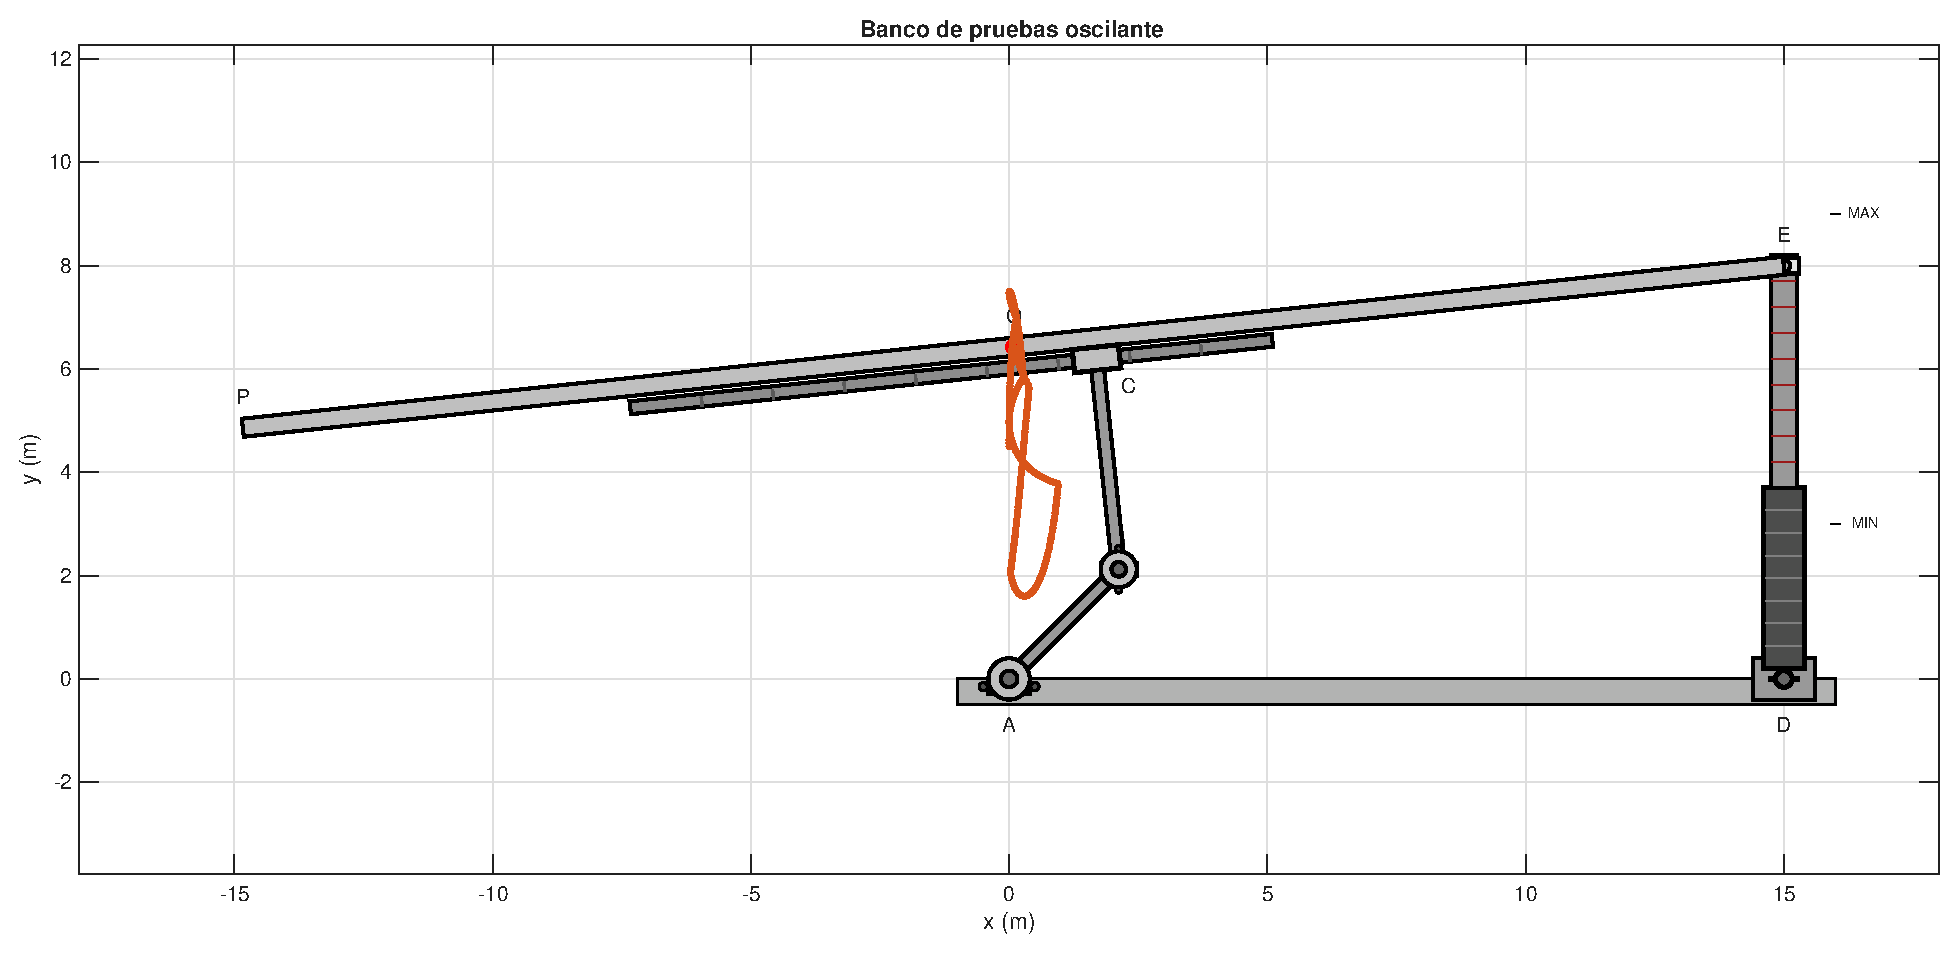
\includegraphics[width=1\textwidth]{images/sim_mechanism.eps}
\caption{Simulación del movimiento del mecanismo en MATLAB}
\label{fig:sim_mechanism}
\end{center}
\end{figure}

El modelo simulado permitió obtener las posiciones relativas de cada eslabón en función del tiempo, calculando además las velocidades y aceleraciones lineales y angulares correspondientes. La trayectoria del punto medio de la barra PE, destacada en color anaranjado, confirma el comportamiento oscilante esperado y evidencia la precisión geométrica del sistema ante diferentes posiciones de entrada.

Los resultados de la simulación coinciden con los valores teóricos obtenidos en el análisis cinemático y cinético del sistema, lo cual valida el modelo implementado y respalda la coherencia de su comportamiento dinámico. Esta correspondencia entre teoría y simulación garantiza la viabilidad del diseño propuesto para su posterior validación experimental.

A partir del modelo cinemático del mecanismo de cinco barras propuesto, se realizaron simulaciones en un entorno computacional para analizar el comportamiento del sistema bajo condiciones de entrada configurables. En esta etapa, se estudiaron cuatro variables principales: la posición angular del eslabón oscilante $\theta_4$, la posición y velocidad del punto medio $O$ de la barra $PE$, y la trayectoria completa del mecanismo durante su operación.

\begin{figure}[H]
\centering
\includegraphics[width=1\textwidth]{images/sim_theta4.eps}
\caption{Posición angular $\theta_4$ vs tiempo}
\label{fig:theta4}
\end{figure}

En la Figura~\ref{fig:theta4} se muestra la evolución de la posición angular $\theta_4$ del eslabón 4 (barra $EP$), correspondiente a la plataforma que soporta la carga. Se observa un patrón \textit{periódico complejo} con oscilaciones entre aproximadamente 163° y 206° a lo largo de 4 segundos de simulación. El comportamiento presenta variaciones de amplitud en cada ciclo, evidenciando la naturaleza no lineal del mecanismo bajo el efecto combinado del movimiento de entrada de la manivela y la acción del actuador telescópico. Los picos de aproximadamente 206° ocurren de manera periódica, con valles intermedios que alcanzan mínimos de alrededor de 164°, confirmando que el sistema genera un movimiento angular cíclico controlado que permite caracterizar el rango de oscilación de la plataforma.

\begin{figure}[H]
\centering
\includegraphics[width=1\textwidth]{images/sim_pos_o.eps}
\caption{Posición del punto $O$ vs tiempo}
\label{fig:posP}
\end{figure}

En la Figura~\ref{fig:posP} se representa la posición del punto $O$ (punto medio de la barra $PE$) en el plano cartesiano, es decir, las coordenadas $P_x (t)$ y $P_y (t)$ a lo largo del tiempo. Se observa que la \textit{coordenada vertical} $P_y$ (línea morada) oscila con amplitud considerable entre aproximadamente 1.5 m y 7.5 m, presentando un patrón sinusoidal característico que refleja el movimiento oscilante principal del sistema. En contraste, la \textit{coordenada horizontal} $P_x$ (línea azul) permanece cerca del origen con oscilaciones de menor amplitud (entre -0.2 m y 1.5 m), lo cual indica que el movimiento dominante es vertical. Los máximos de $P_y$ coinciden aproximadamente con los valores mínimos de$P_x$, revelando una correlación entre ambas componentes que define la trayectoria elíptica del punto $O$. Esta gráfica permite visualizar la trayectoria descrita por el punto medio de la barra $PE$ del mecanismo, información relevante tanto para validar la cinemática como para el posterior análisis dinámico y experimental del banco de pruebas. 

\begin{figure}[H]
\centering
\includegraphics[width=1\textwidth]{images/sim_vel_o.eps}
\caption{Velocidad del punto $O$ vs tiempo}
\label{fig:velP}
\end{figure}

La Figura~\ref{fig:velP} presenta la velocidad del punto $O$ descompuesta en sus componentes horizontal ($V_x$, línea cian) y vertical ($V_y$, línea magenta). Se aprecia que la componente vertical presenta una \textit{oscilación de mayor amplitud}, con valores que varían entre aproximadamente -15 m/s y +20 m/s, mostrando cambios bruscos de dirección que corresponden a los puntos de inversión del movimiento. La componente horizontal $V_x$ exhibe oscilaciones de menor magnitud (entre -7 m/s y +7 m/s aproximadamente), con un comportamiento más irregular debido a la configuración cinemática del mecanismo. Las discontinuidades observadas en las curvas de velocidad están relacionadas con las posiciones singulares o de cambio de configuración del sistema. Esto indica que el movimiento dominante del punto extremo es vertical, lo cual concuerda con el tipo de trayectorias generadas por la configuración tipo \textit{inverted slider-crank}. 

En conjunto, estas tres simulaciones permiten comprobar que el modelo propuesto reproduce de manera consistente el comportamiento oscilante del mecanismo, sirviendo como etapa previa de validación para el diseño mecánico, antes de su implementación física.

\section{Interfaz de Usuario Web}
Como resultado de la implementación descrita en el Marco Metodológico, se obtuvo una interfaz web completamente funcional accesible a través de WiFi desde cualquier dispositivo con navegador web. Esta interfaz constituye la herramienta principal de control y monitoreo del banco de pruebas oscilante.
\begin{figure}[H]
	\centering
	\includegraphics[width=1\textwidth]{images/interfaz.png}
	\caption{Interfaz web implementada para control del banco de pruebas oscilante}
	\label{fig:interfaz}
\end{figure}
La Figura~\ref{fig:interfaz} muestra la interfaz implementada, dividida en dos paneles principales: el generador de ondas (izquierda) y el control de motores (derecha).
\subsection{Panel Generador de Ondas}
El panel izquierdo permite crear patrones de excitación mediante la suma de componentes sinusoidales. En la configuración mostrada:
\begin{itemize}
	\item \textbf{Visualización gráfica superior}: Presenta en tiempo real las dos componentes individuales (líneas semi-transparentes) y la onda resultante (línea gruesa oscura). Un indicador vertical marca el valor instantáneo.
	\item \textbf{Componente 1} (azul): Configurada como seno con amplitud de 50 unidades y frecuencia de 1.0 Hz, se encuentra activa según indica el checkbox marcado.
	
	\item \textbf{Componente 2} (roja): Configurada como seno con amplitud de 30 unidades y frecuencia de 2.0 Hz, también activa.
	
	\item \textbf{Fórmula dinámica}: Muestra la ecuación resultante: 
	
	$y(t) = 50 \cdot \sin(1.0 \cdot t + 0°) + 30 \cdot \sin(2.0 \cdot t + 0°)$
	
	\item \textbf{Valores calculados en tiempo real}:
	\begin{itemize}
		\item Valor Y Total: 20.62 (valor instantáneo de la señal)
		\item Amplitud Máxima: 80 (suma de amplitudes activas)
		\item Tiempo: 63.97 s (contador de simulación)
		\item Componentes Activas: 2
	\end{itemize}
\end{itemize}
La interfaz permite agregar hasta 10 componentes simultáneos mediante el botón "+ Agregar", y eliminar componentes individuales según sea necesario. La velocidad de animación está configurada en 50 unidades en la captura mostrada.
\subsection{Panel Control de Motores}
El panel derecho proporciona controles independientes para ambos actuadores del sistema:
\subsubsection{Motor Rotacional}
Controla la manivela del mecanismo. En la configuración mostrada:
\begin{itemize}
	\item Velocidad: 60 RPM
	\item Dirección: Horario (CW/CCW)
	\item Indicador visual circular animado que refleja el estado actual
\end{itemize}
\subsubsection{Motor Lineal}
Controla el actuador telescópico vertical. Los parámetros visibles son:
\begin{itemize}
	\item Rango de operación: 100 mm (máximo 200 mm)
	\item Velocidad de desplazamiento: 20 mm/s (máximo 100 mm/s)
	\item Posición manual: 0 mm
	\item Modo seleccionado: Manual
	\item Barra gráfica horizontal que muestra visualmente la posición actual
\end{itemize}
Los indicadores de estado en tiempo real muestran:
\begin{itemize}
	\item Posición: 0 mm
	\item Velocidad: 0 mm/s
	\item Estado: Manual
\end{itemize}
El selector de modo permite cambiar entre Manual y Automático según los requerimientos de la prueba.
\subsection{Funcionalidad Demostrada}
La interfaz desarrollada demuestra las siguientes capacidades operativas:
\begin{itemize}
	\item Generación de señales complejas mediante superposición de hasta 10 componentes independientes
	\item Visualización gráfica en tiempo real de las señales generadas
	\item Control independiente de dos motores con parámetros ajustables
	\item Cálculo automático de valores derivados (amplitud máxima, valor instantáneo)
	\item Interfaz responsive accesible desde múltiples dispositivos simultáneamente
	\item Actualización inmediata de todos los parámetros sin necesidad de reiniciar el sistema
\end{itemize}
Esta herramienta permite configurar desde patrones de excitación simples de una sola frecuencia hasta señales complejas multicomponente, facilitando el estudio de la respuesta dinámica del banco de pruebas bajo diversas condiciones de operación controladas.
%% ============================================================================
\renewcommand{\bibname}{\hfill\Large\bf{REFERENCIAS BIBLIOGRÁFICAS}\hfill}

\bibliographystyle{IEEEtran} % Estableciendo el estilo de citas IEEEtram.

\bibliography{referencias} % Recibe las referencias de IEEE

\chapter*{\center \Large ANEXOS} 
\addcontentsline{toc}{section}{\bfseries ANEXOS} 
\markboth{ANEXOS}{ANEXOS} 

\section{Requerimientos de diseño generales}
\label{ANEXO:1}

\begin{longtable}{|>{\raggedright\arraybackslash}p{4cm}|>{\raggedright\arraybackslash}p{11cm}|}
\caption{Requerimientos de diseño generales del banco de pruebas oscilante}
\label{tab:requerimientos_diseno} \\
\hline
\textbf{Requerimiento} & \textbf{Descripción} \\
\hline
\endfirsthead

\multicolumn{2}{c}%
{{\bfseries Continuación de la Tabla \thetable}} \\

\hline
\textbf{Requerimiento} & \textbf{Descripción} \\
\hline
\endhead

\endfoot

\hline
\endlastfoot

Función principal & El banco debe generar oscilaciones mecánicas controladas con amplitud regulable y permitir la adquisición de datos mediante acelerómetros. \\
\hline
Configuración mecánica & El sistema debe tener dos grados de libertad y permitir ajustes de amplitud mediante un mecanismo tipo \textit{inverted slider–crank} con actuador lineal final. \\
\hline
Sensado y adquisición & Debe incorporar sensores inerciales MEMS (como el MPU6050) conectados al microcontrolador ESP32, capaz de adquirir datos a 80 Hz o más. \\
\hline
Interfaz de usuario & La interfaz (desarrollada en ESP32) debe permitir configurar duración, frecuencia de prueba y visualizar datos en tiempo real. \\
\hline
Aplicación académica & El prototipo será de uso en laboratorio educativo. Su diseño debe ser seguro, accesible y confiable para pruebas repetitivas. \\
\hline
Durabilidad & Componentes mecánicos y sensores deben resistir al menos 6 meses de uso académico sin mantenimiento intensivo. \\
\hline
Mantenimiento & El sistema debe ser de fácil desmontaje, limpieza y reemplazo de sensores o piezas críticas. \\
\hline
Condiciones de operación & Uso en ambientes controlados: laboratorio cerrado, temperatura ambiente estable. No expuesto a humedad, viento ni cargas externas pesadas. \\


\end{longtable}


\section{Estructura de funciones}
\label{ANEXO:2}

\subsection{Caja negra con entradas y salidas}

\begin{justify}
Para comprender el funcionamiento del banco de pruebas oscilante desarrollado, se recurre al modelo de caja negra, una herramienta común en ingeniería para representar los sistemas desde el punto de vista funcional, sin detallar su estructura interna. En este modelo, se identifican claramente las entradas, las salidas y el tipo de interacción que mantienen con el sistema.

Cada entrada o salida ha sido clasificada con una letra que indica su naturaleza, según la siguiente nomenclatura:\begin{justify}
Para comprender el funcionamiento del banco de pruebas oscilante desarrollado, se recurre al modelo de caja negra, una herramienta común en ingeniería para representar los sistemas desde el punto de vista funcional, sin detallar su estructura interna. En este modelo, se identifican claramente las entradas, las salidas y el tipo de interacción que mantienen con el sistema.

Cada entrada o salida ha sido clasificada con una letra que indica su naturaleza, según la siguiente nomenclatura:
\begin{itemize}
  \item \textbf{(S)}: Señal — información digital o analógica que circula dentro del sistema, como parámetros configurados desde la interfaz de usuario, datos de sensores o comandos de control.
  \item \textbf{(E)}: Energía — corresponde a las fuentes eléctricas necesarias para el funcionamiento de los componentes del sistema, como el myRIO o el actuador.
  \item \textbf{(M)}: Movimiento o mecánico — se refiere a variables físicas, como el desplazamiento del mecanismo, las fuerzas aplicadas o las condiciones de carga.
\end{itemize}
\end{justify}


\begin{figure}[H]
\centering
\begin{tikzpicture}[node distance=0.8cm and 0.8cm, every node/.style={font=\small}]
  % Caja negra
  \node[draw, fill=black, text=white, align=center, minimum width=5cm, minimum height=9cm] (caja)
{Banco de pruebas oscilante \\ con adquisición basada en \\ acelerómetros};


  % Entradas
  \node[left=of caja, yshift=2.8cm, align=right] (e1) {Energía eléctrica  (Alimentación \\ del controlador) (E)};

  \node[left=of caja, yshift=0.8cm, align=right] (e2) {Señal de control para el \\ motor (S)};

  \node[left=of caja, yshift=-1.5cm,align=right] (e3) {Posicion de actuador \\ lineal (M)};

\node[left=of caja, yshift=-3.2cm,align=right] (e4) {Aceleración angular \\ de la base (S)};

  % Salidas
  \node[right=of caja, yshift=2.8cm] (s1) {Oscilación generada (M)};
  \node[right=of caja, yshift=1.2cm] (s2) {Señales de aceleración (S)};
  \node[right=of caja, yshift=-0.6cm] (s3) {Frecuencia medida (S)};
  \node[right=of caja, yshift=-2.2cm] (s5) {Curva espectral (S)};
  

  % Flechas
\foreach \i in {1,...,4}
\draw[->] (e\i) -- (caja.west|-e\i);
\foreach \i in {1,2,3,5}
\draw[->] (caja.east|-s\i) -- (s\i);

\end{tikzpicture}
\caption{Caja negra con entradas y salidas del banco de pruebas oscilante}
\label{fig:caja_negra_banco}
\end{figure}



La Figura~\ref{fig:caja_negra_banco} representa de manera esquemática el sistema bajo estudio. En cuanto a las entradas, el banco requiere una fuente de alimentación eléctrica, señales de configuración y condiciones físicas impuestas sobre el mecanismo, como la carga o el actuador lineal. Estas entradas permiten definir la duración de la prueba, la frecuencia de oscilación y la amplitud deseada.

Respecto a las salidas, el sistema entrega datos relacionados con el comportamiento dinámico del mecanismo: señales de aceleración obtenidas mediante sensores MEMS, la frecuencia y amplitud resultantes, así como la correspondiente curva espectral calculada. Estos datos son visualizados y exportados para su análisis en tiempo real o posterior.

Este modelo de caja negra facilita la comprensión del flujo de energía, señales e interacción mecánica dentro del sistema, permitiendo un enfoque modular y replicable en futuros desarrollos experimentales.


\subsection{Estructura de funciones global}

\begin{figure}[H]
\centering
\includegraphics[width=1.1\textwidth]{images/vdi.jpg}
\caption{Estructura de funciones global}
\label{fig:estructura_funciones_banco}
\end{figure}


El sistema representado en la Figura~\ref{fig:estructura_funciones_banco} 
 muestra la interacción entre diversos subsistemas diseñados para generar, medir y procesar oscilaciones mecánicas controladas. En primer lugar, el módulo de sensado capta la respuesta dinámica del sistema mediante señales que registran el comportamiento del mecanismo en movimiento. Estas señales representan la aceleración experimentada por el conjunto mecánico y permiten obtener una representación precisa del fenómeno oscilatorio bajo condiciones de prueba definidas.

La información captada por el sensor es recibida por un entorno de interfaz que permite al usuario configurar ciertos parámetros del sistema. A través de esta interfaz, es posible establecer condiciones específicas para cada ensayo, controlar el inicio y la detención del proceso, así como visualizar las variables dinámicas en tiempo real. Este entorno ha sido pensado para favorecer la interacción del estudiante con el sistema físico, permitiendo una experiencia directa con la configuración y supervisión de pruebas dinámicas.

Una vez adquiridas, las señales pasan por un módulo de procesamiento que mejora la calidad de los datos al filtrar posibles perturbaciones o ruidos externos. Este subsistema también transforma la información en un formato más claro y útil para el análisis posterior, permitiendo observar tendencias, identificar comportamientos oscilatorios dominantes y registrar los resultados de cada prueba de forma estructurada. También se incluyen protecciones eléctricas que garantizan la integridad del sistema durante la operación.

La energía para el funcionamiento del sistema se distribuye a través de un circuito regulado que garantiza niveles seguros de alimentación para cada uno de los módulos. Este subsistema incluye protecciones que evitan daños en caso de sobrecarga o mal funcionamiento, asegurando un entorno confiable y seguro para el desarrollo de pruebas continuas. La arquitectura energética fue diseñada para ser estable, autónoma y adecuada para sesiones prácticas dentro de laboratorios educativos.

La señal de control emitida por el sistema se dirige a un mecanismo de accionamiento que transforma la entrada eléctrica en un movimiento periódico. Este movimiento se transfiere hacia el conjunto mecánico, generando una oscilación controlada cuyo comportamiento puede ser modificado en función de los parámetros de entrada. De este modo, es posible observar cómo responde el sistema ante distintas condiciones de operación, lo cual es clave para evaluar su desempeño estructural y dinámico.

El conjunto mecánico, por su parte, está formado por una estructura diseñada para reproducir un movimiento oscilante con solo 2 grados de libertad. Asimismo, su última articulación prismática permite regular la amplitud de la oscilación del mecanismo.













\subsection{Elaboración de alternativas}

Con el objetivo de definir la configuración óptima del banco de pruebas oscilante, se plantearon tres alternativas combinando distintos componentes para cumplir con las funciones clave del sistema. Estas combinaciones se basaron en la matriz morfológica de la tabla~\ref{tab:matriz_morfologica}, donde se establecen opciones viables para cada función del sistema. A continuación, se detallan las alternativas propuestas:

\begin{itemize}
    \item \textbf{Alternativa 1 (Propuesta final en esta tesis):} \\
    1C - 2A - 3B - 4A - 5A - 6A

    \item \textbf{Alternativa 2:} \\
    1B - 2A - 3A - 4A - 5C - 6C

    \item \textbf{Alternativa 3:} \\
    1A - 2B - 3B - 4B - 5A - 6A
\end{itemize}

{\small
\begin{longtable}[H]{|>{\centering\arraybackslash}m{4cm}|p{3.6cm}|p{3.6cm}|p{3.6cm}|}
\caption{Matriz morfológica del sistema propuesto con imágenes}
\label{tab:matriz_morfologica}
\\ \hline
\textbf{Función} & \textbf{Opción A} & \textbf{Opción B} & \textbf{Opción C} \\
\hline
\endfirsthead

\hline
\textbf{Función} & \textbf{Opción A} & \textbf{Opción B} & \textbf{Opción C} \\
\hline
\endhead

\hline
\multicolumn{4}{r}{\textit{}} \\
\endfoot

\hline
\endlastfoot


(1) Regular amplitud de oscilación &
\makecell{\includegraphics[width=0.6\linewidth]{images/2.png} \\ Actuador lineal\\ Sawers} &
\makecell{\includegraphics[width=0.6\linewidth]{images/3.png} \\ Actuador lineal\\ SFU1605} &
\makecell{\includegraphics[width=0.6\linewidth]{images/propio.png} \\ Diseño propio\\ ajustable}\\
\hline

(2) Medir aceleración &
\makecell{\includegraphics[width=0.8\linewidth]{images/3A.jpg} \\ MPU6050} &
\makecell{\includegraphics[width=0.8\linewidth]{images/3B.jpg} \\ ADXL345} &
\makecell{\includegraphics[width=0.8\linewidth]{images/3C.jpeg} \\ ISM330DHCX} \\
\hline

(3) Controlador de adquisición &
\makecell{\includegraphics[width=0.6\linewidth]{images/4A.jpg} \\ NI myRIO} &
\makecell{\includegraphics[width=0.8\linewidth]{images/Imagen1.jpg} \\ ESP32} &
\makecell{\includegraphics[width=0.8\linewidth]{images/4C.jpeg} \\ Raspberry Pi Pico} \\
\hline

(4) Filtrado de señal &
\makecell{Filtro \\ pasa-banda} &
\makecell{Filtro de Kalman} &
\makecell{Ventana móvil} \\
\hline

(5) Interfaz de usuario &
\makecell{ESP32} &
\makecell{MATLAB GUI} &
\makecell{LabView} \\
\hline



\end{longtable}
}


\subsection{Comparación de alternativas}

Para seleccionar la alternativa más adecuada, se evaluaron las opciones propuestas según los criterios técnicos definidos en la Tabla~\ref{tab:criterios_tecnicos}. 

\begin{table}[H]
    \centering

    \begin{tabular}{|p{5cm}|p{9.5cm}|}
        \hline
        \textbf{Criterio} & \textbf{Descripción} \\
        \hline
        Tamaño & Volumen físico ocupado por el sistema en el laboratorio. \\
        \hline
        Robustez & Capacidad del sistema para mantener su funcionamiento bajo condiciones dinámicas (vibraciones, variaciones de carga). \\
        \hline
        Consumo energético & Energía eléctrica utilizada durante una jornada de pruebas. \\
        \hline
        Precisión del sensado & Exactitud y estabilidad de los datos adquiridos por los sensores de aceleración. \\
        \hline
        Disponibilidad & Facilidad de conseguir los componentes en el mercado local y tiempo de adquisición. \\
        \hline
        Facilidad de integración & Facilidad para ensamblar, montar y configurar el sistema completo. \\
        \hline
        Compatibilidad educativa & Nivel de familiaridad y facilidad de uso del sistema para fines de enseñanza y aprendizaje. \\
        \hline
    \end{tabular}
    \caption{Descripción de criterios técnicos}
        
    \label{tab:criterios_tecnicos}
\end{table}

En la tabla~\ref{tab:comparacion_alternativas}, se observa la comparación entre cada alternativa y a cada criterio se le asignó un peso (g) de importancia de 1 a 4 y a cada alternativa un puntaje (p) entre 1 y 4. Se multiplicó cada puntaje por su peso (gp) y se sumaron los resultados para obtener un valor técnico relativo.

\begin{table}[H]
    \centering

    \begin{tabular}{|l|c|c|c|c|c|c|c|c|}
        \hline
        \textbf{Criterio} & \textbf{g} & \textbf{Alt. 1 (p)} & \textbf{gp} & \textbf{Alt. 2 (p)} & \textbf{gp} & \textbf{Alt. 3 (p)} & \textbf{gp} \\
        \hline
        Robustez y estabilidad & 5 & 3 & 15 & 2 & 10 & 2 & 10 \\
        \hline
        Flexibilidad & 3 & 3 & 9 & 3 & 9 & 3 & 9 \\
        \hline
        Facilidad de desarrollo & 3 & 3 & 9 & 2 & 6 & 2 & 6 \\
        \hline
        Baja latencia & 5 & 3 & 15 & 2 & 10 & 3 & 15 \\
        \hline
        Precisión del sensado & 5 & 3 & 15 & 2 & 10 & 2 & 10 \\
        \hline
        Compatibilidad educativa & 4 & 3 & 12 & 3 & 12 & 3 & 12 \\
        \hline
        \textbf{Puntaje máximo} & & & \textbf{75} & & \textbf{57} & & \textbf{62} \\
        \hline
        \textbf{Valor técnico} & & & \textbf{0.75} & & \textbf{0.57} & & \textbf{0.62} \\
        \hline
    \end{tabular}
    \caption{Comparación de alternativas}
    
    \label{tab:comparacion_alternativas}
\end{table}

Se observa que la alternativa 1 presenta el mayor valor técnico (0.88), debido a su robustez, precisión de sensado, alta disponibilidad y compatibilidad con entornos académicos. Por ello, esta alternativa fue seleccionada para el desarrollo del prototipo experimental del banco de pruebas oscilante.





\section{Diagrama de Gantt}

\begin{figure}[H]
\centering
\begin{ganttchart}[
    %time slot unit=week,
    title label font=\bfseries\footnotesize,
    title label anchor/.style={below=-1.5ex},
    bar label font=\small,
    bar/.append style={draw=black},
    x unit=0.6cm,
    y unit chart=0.5cm,
    vgrid,
    hgrid,
    title/.style={fill=gray!20},
    progress label text={}
]{1}{16}
    \gantttitlelist{1,...,16}{1} \\

    % Fase inicial: revisión, ideas, objetivos
    \ganttgroup[bar/.append style={fill=gray!30}]{Fase inicial y planificación}{1}{5} \\
    \ganttbar[bar/.append style={fill=gray!20}]{Revisión bibliográfica}{1}{2} \\
    \ganttbar[bar/.append style={fill=gray!40}]{Ideación del sistema}{2}{3} \\
    \ganttbar[bar/.append style={fill=gray!50}]{Formulación de objetivos y alcances}{3}{4} \\
    \ganttbar[bar/.append style={fill=gray!60}]{Esquema general del documento}{4}{5} \\

    % Capítulo 1: Introducción
    \ganttgroup[bar/.append style={fill=orange!50}]{Capítulo 1: Introducción}{6}{7} \\
    \ganttbar[bar/.append style={fill=orange!40}]{Borrador}{6}{6} \\
    \ganttbar[bar/.append style={fill=orange!60}]{Revisión y correcciones}{7}{7} \\

    % Capítulo 2: Marco Teórico
    \ganttgroup[bar/.append style={fill=teal!50}]{Capítulo 2: Marco Teórico}{8}{13} \\
    \ganttbar[bar/.append style={fill=teal!40}]{Borrador}{8}{9} \\
    \ganttbar[bar/.append style={fill=teal!60}]{Revisión interna}{10}{11} \\
    \ganttbar[bar/.append style={fill=teal!80}]{Revisión final}{12}{13} \\

    % Capítulo 3: Metodología
    \ganttgroup[bar/.append style={fill=blue!50}]{Capítulo 3: Metodología}{12}{16} \\
    \ganttbar[bar/.append style={fill=blue!40}]{Borrador}{12}{14} \\
    \ganttbar[bar/.append style={fill=blue!60}]{Revisión y versión final}{15}{16} \\

    % Línea de progreso actual (semana 11)
    \ganttmilestone[inline=false, milestone label font=\scriptsize\bfseries,
        milestone label node/.append style={left=4pt},
        milestone label text={\scriptsize Semana actual}
    ]{}{11}

\end{ganttchart}
\caption{Cronograma de redacción del informe}
\label{fig:avance_general_cap1a3}
\end{figure}




\section{Tabla de información}

\begin{longtable}{|p{3cm}|p{2cm}|p{6cm}|p{3cm}|}
    \hline
    \textbf{Revista Científica} & \textbf{Cuartil} & \textbf{Información Relevante} & \textbf{Fuente} \\
    \hline
    \endfirsthead

    \hline
    \textbf{Revista Científica} & \textbf{Cuartil} & \textbf{Información Relevante} & \textbf{Fuente} \\
    \hline
    \endhead

    The Journal of Adhesion & Q2 & Analiza experimentalmente la respuesta dinámica de acelerómetros montados con adhesivos estructurales, destacando el impacto del tipo de adhesivo en el rendimiento mediante análisis espectral usando transformada de Fourier. & Cocconcelli, M. y Spaggiari, A. (2015). Mounting of Accelerometers with Structural Adhesives: Experimental Characterization of the Dynamic Response. \\
    \hline

    Machines & Q2 & Presenta un sistema de medición de vibraciones de bajo costo para entornos industriales, validado mediante comparación con sistemas de referencia y análisis con transformada rápida de Fourier y método de Welch. & Villarroel, A., Zurita, G., y Velarde, R. (2019). Development of a Low-Cost Vibration Measurement System for Industrial Applications. \\
    \hline

    IEEE/ASME Transactions on Mechatronics & Q1 & Describe métodos para reducir vibraciones y oscilaciones en un banco de pruebas HiL para dirección, incluyendo modelado dinámico, diseño de control y análisis experimental para mejorar la estabilidad y precisión. & Haas, A., Schrage, B., Menze, G., Sieberg, P. M., Schramm, D. (2024). Oscillation and Vibration Reduction Approaches on a HiL-Steering-Test-Bench. \\
    \hline

    Journal of Robotics and Control (JRC) & Q2 & Desarrolla una plataforma de aislamiento activo de vibraciones usando elastómeros magnetorreológicos, con modelado y diseño de control para mejorar la estabilidad y reducir vibraciones de baja frecuencia. & Mikhailov, V., Kopylov, A., Kazakov, A. (2024). Modeling and Designing of Active Vibration Isolation Platform. \\
    \hline

    23rd ABCM International Congress of Mechanical Engineering–COBEM & Q2 & Diseña un banco de pruebas económico usando componentes reciclados para la enseñanza de técnicas de análisis de vibraciones aplicadas a mantenimiento predictivo, facilitando mediciones prácticas para estudiantes. & Lima, I. A. M., y Nunes, M. A. A. (2015). Design and Construction of a Test Bench for Study of Vibration Analysis Techniques Applied to Predictive Maintenance. \\
    \hline

    European Journal of Engineering Education & Q2 & Analiza la importancia del aprendizaje práctico en laboratorios de ingeniería, enfatizando el rol fundamental de los bancos de pruebas para la formación y la experimentación en ingeniería. & Lima, R., Mesquita, D., y Flores, M. A. (2017). The importance of hands-on learning and the role of engineering education labs. \\
    \hline

    Procedia Computer Science & Q3 & Presenta una plataforma experimental inteligente para mantenimiento predictivo basada en análisis de vibraciones, integrando sensores y procesamiento para anticipar fallas en sistemas industriales. & Guedes, A. P. C., Neves, M. M., y Maran, A. L. R. (2021). A Smart Experimental Platform for Predictive Maintenance Based on Vibration Analysis. \\
    \hline

Mechatronics Journal & Q1 & Este estudio analiza la respuesta dinámica de una articulación robótica bajo cargas oscilantes. Los resultados obtenidos permiten comprender el comportamiento del sistema frente a vibraciones mecánicas. & Y. Chen, X. Ma, and Z. Liu, “Dynamic response analysis of a robotic joint under oscillatory loads,” Mechatronics Journal, vol. 45, no. 3, pp. 223–230, 2020. \\
    \hline

Journal of Biomechatronics & Q2 & Simula la oscilación de miembros robóticos mediante actuadores neumáticos. Los datos obtenidos permiten caracterizar las respuestas dinámicas de sistemas oscilantes en condiciones biológicas. Esto proporciona un marco de comparación para validación de plataformas similares en sistemas mecatrónicos. & K. Fujimoto, M. Takeda, and A. Sato, “Simulation of limb oscillations using pneumatic actuation in biomechatronic testbeds,” Journal of Biomechatronics, vol. 10, no. 2, pp. 112–120, 2021. \\
    \hline

IEEE Trans. Control Syst. Tech. & Q1 & Evalúa la robustez de controladores a través de un péndulo invertido sometido a oscilaciones. La metodología utilizada ofrece parámetros clave para pruebas bajo excitación controlada. & J. López-Linares, D. Rojas, and F. Méndez, “Control robustness testing via oscillations in an inverted pendulum system,” IEEE Transactions on Control Systems Technology, vol. 30, no. 1, pp. 98–107, 2022. \\
    \hline

Robotics and Autonomous Systems & Q1 & Diseña una plataforma robótica experimental con oscilaciones adaptativas para probar algoritmos de amortiguamiento. La plataforma validó con éxito estrategias de control robusto. & T. Rahman, S. Ali, and N. Chowdhury, “Adaptive damping in oscillatory robotic systems: Experimental platform design and testing,” Robotics and Autonomous Systems, vol. 118, pp. 43–51, 2019. \\
    \hline

IEEE/ASME Trans. Mechatronics & Q1 & Presenta una plataforma oscilatoria de 1 DOF equipada con acelerómetros MEMS, validando su capacidad para medir microoscilaciones. Apoya directamente la elección tecnológica del sistema de adquisición en el proyecto propuesto. & H. Lin, J. Wu, and Y. Zhao, “Design and characterization of a 1-dof oscillatory platform using mems accelerometers,” IEEE/ASME Transactions on Mechatronics, vol. 25, no. 3, pp. 1453–1461, 2020. \\
    \hline

IEEE Trans. Ind. Electronics & Q1 & Evalúa microoscilaciones en actuadores robóticos utilizando acelerómetros piezoeléctricos. El estudio demuestra sensibilidad y fidelidad de estos sensores. Refuerza la elección de acelerómetros como sensores en bancos de prueba dinámicos. & L. Zhang, Y. Chen, and C. Lee, “Experimental evaluation of micro-oscillations in robotic actuators using piezoelectric accelerometers,” IEEE Transactions on Industrial Electronics, vol. 63, no. 6, pp. 3445–3453, 2016. \\
    \hline

IEEE/ASME Trans. Mechatronics & Q1 & Integra retroalimentación en tiempo real con acelerómetros MEMS y microcontroladores STM32 en sistemas de suspensión activa. Muestra la aplicabilidad de sistemas embebidos en adquisición dinámica, útil para el diseño del sistema propuesto. & S. Jang, H. Kim, and Y. Park, “Real-time oscillation feedback in active suspension systems using stm32 and mems accelerometers,” IEEE/ASME Transactions on Mechatronics, vol. 27, no. 3, pp. 1805–1812, 2022. \\
    \hline

Int. J. Mechatronics Education & Q3 & Propone un sistema de bajo costo para la enseñanza de oscilaciones mecánicas usando sensores MEMS. Aporta ideas de diseño accesible y educativo para el banco oscilante con fines experimentales. & R. Martínez-Castro, S. Flores et al., “Low-cost experimental setup for teaching mechanical oscillations with mems accelerometers,” International Journal of Mechatronics Education, vol. 12, no. 1, pp. 25–34, 2021. \\
    \hline

IEEE Transactions on Mechatronics & Q1 & Valida algoritmos de control robusto usando una plataforma de excitación mecánica controlada. El diseño demuestra cómo la excitación puede ser replicada para evaluación de controladores, aplicable a pruebas experimentales similares. & A. Müller, B. Schneider, and M. Hofmann, “Experimental validation of robust control algorithms using controlled mechanical excitation,” IEEE Transactions on Mechatronics, vol. 26, no. 4, pp. 2145–2153, 2021. \\
    \hline

J. Dyn. Sys., Meas. and Control & Q2 & Emplea excitación mecánica PID para caracterizar parámetros dinámicos en bancos oscilantes. Relevante para el diseño de controladores en el banco de pruebas planteado. & H. Tanaka, K. Saito, and R. Inoue, “Pid-controlled mechanical excitation for system parameter identification in oscillating testbeds,” Journal of Dynamic Systems, Measurement, and Control, vol. 141, no. 2, p. 021005, 2019. \\
    \hline

Mechatronics & Q1 & Describe un sistema servoaccionado para pruebas de fatiga estructural con cargas oscilantes. El sistema es altamente adaptable y puede ser replicado para validar modelos dinámicos. & C. Delgado, L. Vargas, and J. Méndez, “Adaptive servo-driven excitation system for structural fatigue testing in mechatronic components,” Mechatronics, vol. 68, p. 102364, 2020. \\

    \hline

IJERI & Q3 & Desarrolla un banco oscilante de bajo costo con motores paso a paso para validar sensores MEMS. & R. Morales-Torres, F. Gutiérrez, and D. Ruiz, “Low-cost oscillating bench using stepper motors for experimental validation of mems sensors,” International Journal of Engineering Research and Innovation, vol. 24, no. 1, pp. 33–40, 2022. \\
    \hline

IEEE/ASME Trans. Mechatronics & Q1 & Diseña un banco oscilatorio 1 DOF para estructuras flexibles. Su enfoque experimental y validación es directamente aplicable a plataformas similares para caracterizar comportamiento dinámico. & L. Chen, J. Zhang, and H. Wei, “Design of a 1-dof oscillatory test bench for dynamic analysis of flexible structures,” IEEE/ASME Transactions on Mechatronics, vol. 26, no. 3, pp. 2120–2129, 2021. \\

    
    \hline

    \caption{Tabla de Información de revistas}
\end{longtable}



\end{document}
